\documentclass[]{MSword}
% Class options:
%-------------------------------
% nobib         - skip bibliography code/ don't include bib
% math          - include math packages and useful math commands
% hidelinks     - hide hyperref colored link boxes
% wordlinks     - link color scheme similar to word


% Preamble code:
%%%%%%%%%%%%%%%%%%%%%%%%%%%%%%%%%%%%%%%%
\usepackage[english]{babel}
\usepackage{csquotes}
\usepackage{textcomp}
\usepackage{comment}
\usepackage{listings}
\usepackage{graphicx}
\usepackage{caption}
\usepackage{subcaption}

\definecolor{codegreen}{rgb}{0,0.6,0}
\definecolor{codegray}{rgb}{0.5,0.5,0.5}
\definecolor{codepurple}{rgb}{0.58,0,0.82}
\definecolor{backcolor}{rgb}{0.95,0.95,0.92}
 
\lstdefinestyle{mystyle}{
    backgroundcolor=\color{backcolor},   
    commentstyle=\color{codegreen},
    keywordstyle=\color{magenta},
    numberstyle=\tiny\color{codegray},
    stringstyle=\color{codepurple},
    basicstyle=\footnotesize,
    breakatwhitespace=false,         
    breaklines=true,                 
    captionpos=b,                    
    keepspaces=true,                 
    numbers=left,                    
    numbersep=5pt,                  
    showspaces=false,                
    showstringspaces=false,
    showtabs=false,                  
    tabsize=2
}
\lstset{emph={%  
    as, True, False%
    },emphstyle={\color{magenta}}%
}%
 
\lstset{style=mystyle}




% % Uncomment using "Ctrl + /" (/ on numpad):
% % Customizing headers and footers:
% \fancypagestyle{custom}{%
%     \fancyhf{}% clears the footer and header
%     % Header:
%     \fancyhead[L]{}
%     \fancyhead[C]{}
%     \fancyhead[R]{}
%     % Footer:
%     \fancyfoot[L]{}
%     \fancyfoot[C]{}
%     \fancyfoot[R]{}
%         % Tips:
%         % ----
%         % L: left, C: center, R: right
%         % O: odd pages, E: even pages
%         % ----
%         % Example: \fancyghead[LO,RE]{Text}
%         % will produce "Text" left in the header
%         % on odd pages and right in the header on even pages.
%     % Rules/ lines:
%     \renewcommand{\headrulewidth}{0.4pt}
%     \renewcommand{\footrulewidth}{2pt}
% }
% % Changing the pagestyle:
% \pagestyle{custom}

%%%%%%%%%%%%%%%%%%%%%%%%%%%%%%%%%%%%%%%%

% Preamble information:
%%%%%%%%%%%%%%%%%%%%%%%%%%%%%%%%%%%%%%%%

\title{Abschlussarbeit 

"Anpassbarer Construktionsplaner mit automatischer Bauplandeduktion (ACAB)"}
\author{Sebastian Rossi}
\date{January 2023}

%%%%%%%%%%%%%%%%%%%%%%%%%%%%%%%%%%%%%%%%

% The document:
%%%%%%%%%%%%%%%%%%%%%%%%%%%%%%%%%%%%%%%%
\begin{document}
\maketitle
%\begin{center}
%    Words: \quickwordcount{main}\\ % Word count 
%    Pages: \pageref{LastPage} % Page count
%\end{center}

% Text files from txt folder:
\chapter{Motivation}\label{motivation}
Der stetig steigende Fachkräftemangel trifft auch das Baugwerbe. 
Laut einer Umfrage des Hauptverbandes der Deutschen Bauindustrie e.V. stufen über 75 Prozent aller befragten Unternehmen sowohl den vorherrschenden Fachkräftemangel, als auch die steigenden Energie- und Rohstoffpreise als Risiko für das eigene wirtschaftliche Wachstum ein \cite{Bauindustrie:online}.
Abbildung~\ref{fig:Fachkraeftemangel} illustriert die Entwicklung dieser Sorge über einen Zeitraum von etwas mehr als zwanzig Jahren.
Damit ist es wenig überraschend, dass eine Bewegung weg von menschlichen Arbeitskräften hin zur Automatisierung existiert.
Neben dem Fachkräftemangel stellt aber auch die geringe Effizienz von Bauvorhaben ein Problem dar, welche sich über den gesamten Planungs- und Bauprozess erstreckt. 
Diese Ineffizienz entsteht aufgrund der Vielzahl der an Bauprojekten beteiligten Experten und Unternehmen.
Dies ist ein bekanntes Problem und wird als \textit{Fragmentierungsproblem der Bauindustrie} bezeichnet~\cite{ConstructionFragmentation}.
\begin{figure}[h]
    \centering
    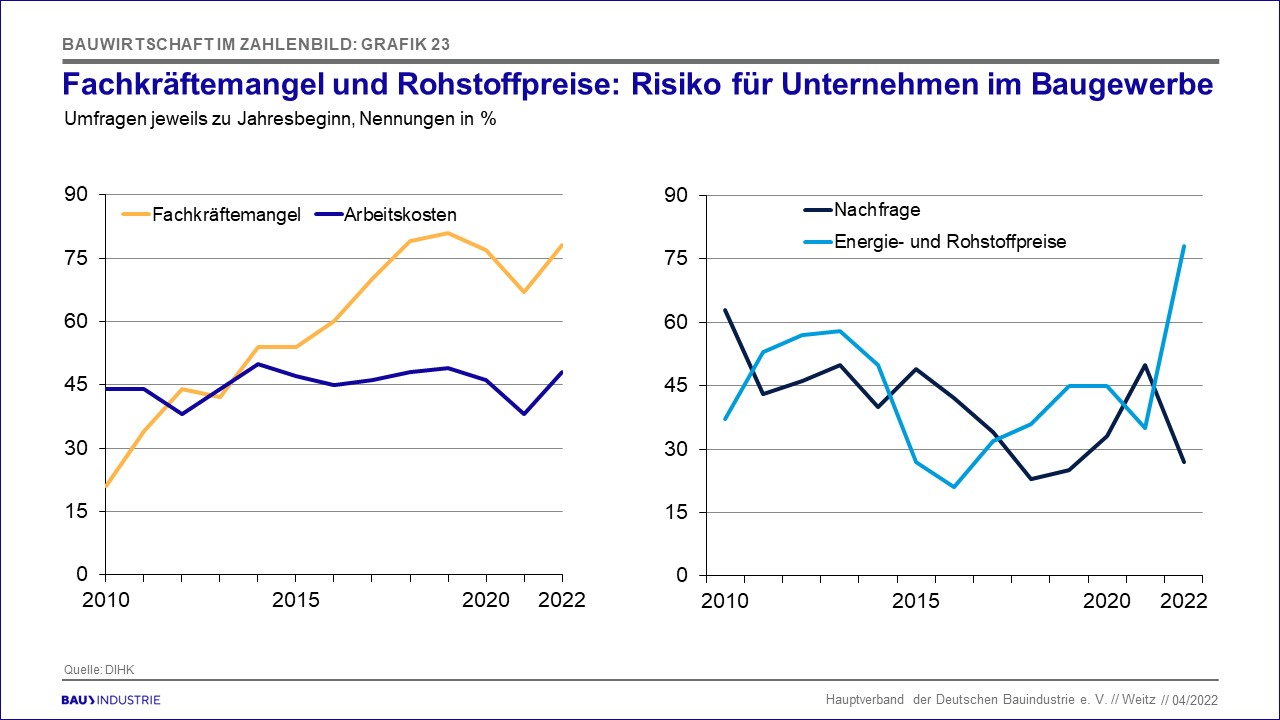
\includegraphics[width=0.7\columnwidth]{fig/Grafik_23.jpg}
    \caption{Während wirtschaftliches Risiko durch eine potentiell sinkende Nachfrage nach Bauafträgen und eventuell steigender Arbeitskosten unverändert blieben oder sogar als weniger relevant bewertet wurden, ist ein deutlicher Anstieg aufgrund des vorherrschenden Fachkräftemangels und der Energie- und Rohstoffpreise zu erkennen.}
    \label{fig:Fachkraeftemangel}
\end{figure}
Um dem entgegenzuwirken, etablieren sich bereits seit einigen Jahren Standards, um Bauprojekte digital zu begleiten.
Mit diesen soll gleichzeitig die Effizienz gesteigert, die Kommunikation zwischen den einzelnen Expertenteams vereinfacht, der Arbeitsplatz \glqq{}Baustelle\grqq{} sicherer gestaltet und ein resourcensparender Bau ermöglicht werden~\cite{BIMforHe12:online}\cite{Top10Ben31:online}.
Zusätzlich steigen mit der Zunahme an digitalen Informationen zu Bauprojekten, auch die Möglichkeiten diese ausführlicher zu analysieren, zu optimieren und an neue Technologien zu knüpfen.
Erst dadurch wurde das seit einigen Jahren erforschte Gebiet der \textit{Additiven Fertigung} von Gebäuden realisierbar.
Einige erfolgreiche Beispiele dafür sind in~\cite{AdditiveManufactoringDelgado},~\cite{AdditiveManufacturingUsingMobileRobots} und~\cite{Tankova2020} aufgezeigt und wurden etwa mit Beton druckenden Roboterarmen, mobilen Robotern oder aufgehängten Druckköpfen durchgeführt.
Dabei werden teils herkömmliche, teils speziell für die druckenden Roboter entwickelte Materialien verwendet~\cite{Tankova2020}.
Obwohl es mittlerweile viele Projekte zur Additiven Fertigung von Gebäuden gibt, haben diese oft den Nachteil der Nicht-Parallelisierbarkeit der druckenden Roboter und die daraus resultierende, vergleichsweise lange Bauzeit.
Auch die durch die Höhe der temporären Stützstrukturen (wie Kräne, Gerüste oder Aufhängungen) eingeschränkte Bauhöhe limitiert die Vielfalt der mit additiver Fertigung realisierbaren Projekte.
Diesen Einschränkungen soll nun mithilfe eines Schwarmes bodengebundener automoner Roboter, die gleichzeitig an dem Bauprojekt arbeiten können, entgegengewirkt werden.
Dabei sollen sich die Roboter auf den Mauern des Gebäudes selbst bewegen können, während sie diese errichten.
Im Gegensatz zur additiven Fertigung sollen die Roboter das Material nicht etwa drucken, sondern herkömmliche Bausteine verweden können.
In dieser Arbeit liegt der Schwerpunkt allerdings nicht auf der Entwicklung dieser Roboter, sondern auf dem Erarbeiten eines Vorgehens zur Berechnung von für Roboterschwärme geeigneten Bauplänen, ausgehend von 3D Modellen der Gebäude.
Dies stellt die Grundlage für nachfolgende Automatisierungsprojekte im Bereich der Bauindustrie dar.
Das Anfertigen der Modelle innerhalb eines 3D Editors ermöglicht nicht nur das Definieren geometrischer und physikalischer Eigenschaften eines Gebäudes in digitaler Form, sondern verschlankt zudem die Kommunikation zwischen Endnutzer und Architekturbüro oder ersetzt letzteres komplett.
Gleichzeitig macht diese Arbeit damit einen Schritt in Richtung des relativ neuen Trends der sogennanten Massenpersonalisierung, welcher als Nachfolgetrend zur Massenproduktion und als \glqq{}heilger Gral\grqq{} der Fertigung angesehen wird~\cite{MassCustomHolyGrail}.
Dieser Trend ist auch für die Bauindustrie interessant, denn auch hier schafft die Möglichkeit sämtliche Kundenwünsche an ein Produkt (oder in diesem Fall ein Gebäude) umzusetzen, ohne dafür spezielles Werkzeug herstellen oder Verfahren entwickeln zu müssen, neue Gewinnmöglichkeiten~\cite{Jensen2018}~\cite{Jensen2015}.
Dennoch existiert noch vergleichsweise wenig Forschung die teilweise schon etablierte Konzepte der Massenpersonalisierung aus der Fertigungsindustrie ebenfalls in der Bauindustrie zu erproben~\cite{Larsen2019}.
Darum soll in dieser Arbeit untersucht werden, in welcher Weise sich bereits vorhandene digitale Standards und Austauschformate dafür eigenen, individuelle Baupläne aus den 3D Plänen von Gebäuden zu generieren.
Die Baupläne können dabei aufgrund der Anbindung an einen frei verfügbaren 3D Editor nicht nur von Experten, sondern ebenfalls von Laien stammen.
So kann ein Endnutzer persönliche Wünsche selbst in das Modell integrieren.
Zudem wird nach einer Möglichkeit gesucht, die resultierenden Baupläne durch adaptive Regelsets an die jeweilige Situation anpassen zu können, denn unterschiedliche Bauprojekte besitzen oft unterschiedliche Eigenheiten und Prioritäten.
Diese Konzepte werden daraufhin anhand nachfolgender Fallstudien getestet.
\chapter{Fallstudien}\label{scenarios}
Anhand der nachfolgenden Fallstudien und Szenarien werden die dieser Arbeit zugrundeliegenden Konzepte veranschaulicht und auf Anwendbarkeit überprüft.
Dabei werden die Szenarien zunehmend komplexer, um auch das Zusammenspiel verschiedener Teilkonzepte zur Lösung einzelner Probleme zu verifizieren.
Abschließend wird für einige Szenarien untersucht wie Regeln erstens definiert und zweitens auf deren Ergebnisse angewandt werden können.
Damit sollen die ungeordneten Listen an Bausteinen, die das Ergebnis der Szenarien darstellen, so umsortiert werden, dass daraus ein schrittweise umsetzbarer Bauplan entsteht.

\section{Szenario 1}\label{scenarios:scenario1}
In diesem einleitenden Szenario werden anhand eines einfachen vierwändigen Turmes einige der Kernkonzepte geprüft.
Dabei werden sowohl die Modellierung des Turmes innerhalb eines Konstruktionsplaners, als auch die anschließende Bauplandeduktion thematisiert.
Insbesondere das Anwenden verschiedener Mauerwerksverbände soll die Flexibilität des erarbeiteten Vorgehens demonstrieren.
\subsection*{Beschreibung}
Das Modellieren des Gebäudes soll mit Hilfe der in Kapitel~\ref{basics} näher behandelten Technologien geschehen und enstpricht darum in seiner Struktur einem verbreiteten Industriestandard.
Der Turm besteht lediglich aus vier 20 Meter hohen Wänden, die einen einzigen Raum einschließen.
Es hat einen Grundriss von 10$\times$10 Metern.
Die Wände sollen daraufhin unter Anwendung folgender Mauerwerksverbände realisiert werden:
\begin{itemize}
  \item Einem Läuferverband mit einem Versatz von 50\% der Bausteinlänge.
  \item Einem Kopf/Binderverband.
  \item Einem Kreuzverband 
\end{itemize}
Da die beiden letzten Verbände bei gleichbleibendem Modul die Wanddicke verdoppeln, muss das Modell etwas angepasst werden, um nach wie vor den selben Grundriss aufzuweisen.
Als Basismodul wird ein Baustein mit den Maßen 2$\times$1$\times$0.5 Metern verwendet.
Das vereinfacht die Interpretation der generierten Lösungen.
Das dazugehörige Raster hat die Größe 1$\times$1$\times$0.5 Meter.

\subsection*{Problemstellungen}
Durch Lösen dieser Szenarien werden folgende Fragestellungen beantwortet:
\begin{itemize}
  \item In welcher Art muss das Basismodul vorliegen und wie kann es notfalls angepasst werden? 
  Denn oftmals werden an Wandenden oder Ecken Bausteine benötigt, die eine geringere Länge aufweisen.
  Dies entspricht in Realität dem Zerschneiden von Bausteinen.
  \item Wie können einem Algorithmus die verschiedenen Mauerwerksverbände sinnvoll vorgegeben werden?
  \item Wie können Eckbereiche gefunden und der jeweilige Mauerwerksverband auch an diesen Stellen passend angebracht werden ohne das Überbindemaß (siehe Kapitel~\ref{basics:Mauerwerksverband}) zu verletzen?
  \item Welche Informationen werden in den resultierenden Bauplan integriert?
\end{itemize}

\section{Szenario 2}\label{scenarios:scenario2}
Nun folgt ein Szenario das den Gegebenheiten eines realen Gebäudes eher entspricht.
Es soll ein Gebäude konstruiert werden, welches einen Innenraum, Fenster und Türen enthält.
Gleichzeitig wird das Modul stark verkleinert, sodass es den Maßen eines 4$\times$2 LEGO Steins entspricht (siehe Kapitel~\ref{basics:lego}).

\begin{figure}[ht]
  \centering
  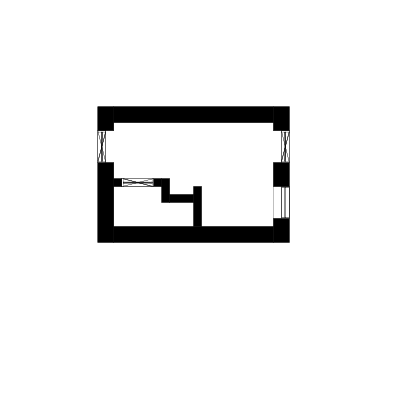
\includegraphics[width=0.505\columnwidth]{fig/scenario1_story_plan.jpg}
  \caption{Gebäudeplan des 3D Modells.}
  \label{fig:scenarios:Scenario1 Gebaeudeplan}
\end{figure}

\subsection*{Beschreibung}
Zu sehen ist der Plan eines einfachen Hauses mit einem Stockwerk.
Dieses besitzt eine Eingangstür, eine Terassentür neben einem Fenster und eine Tür, die das Badezimmer vom Hauptraum trennt.
Türen und Fenster stellen eine Herausforderung für den Planungsalgorithmus dar, da der Verlauf einer ansonsten durchgängigen Wand dadurch unterbrochen wird und Lücken aufweist.
Es gibt breite Außen- und dünne Innenwände.
Dafür müssen zwei Wandtypen definiert werden, die jeweils unterschiedliche Wanddicken vorgeben.
Diese entsprechen in ihren Maßen dem Raster, welches das \textit{LEGO System} vorgibt.
Breite Wände sollen zwei Noppen breit sein.
Daher hat deren Grundmodul Maße von 31.8$\times$15.8$\times$9.6 Millimetern mit einem Raster von 8$\times$8$\times$9.6 Millimetern.
Für die dünneren Innenwände soll eine Breite von einer Noppe verwendet werden.
Dies entspricht einem Grundmodul mit den Maßen 15.8$\times$7.8$\times$9.6 Millimetern mit einem gleichbleibenden Raster.
\begin{figure}[!ht]
  \centering
  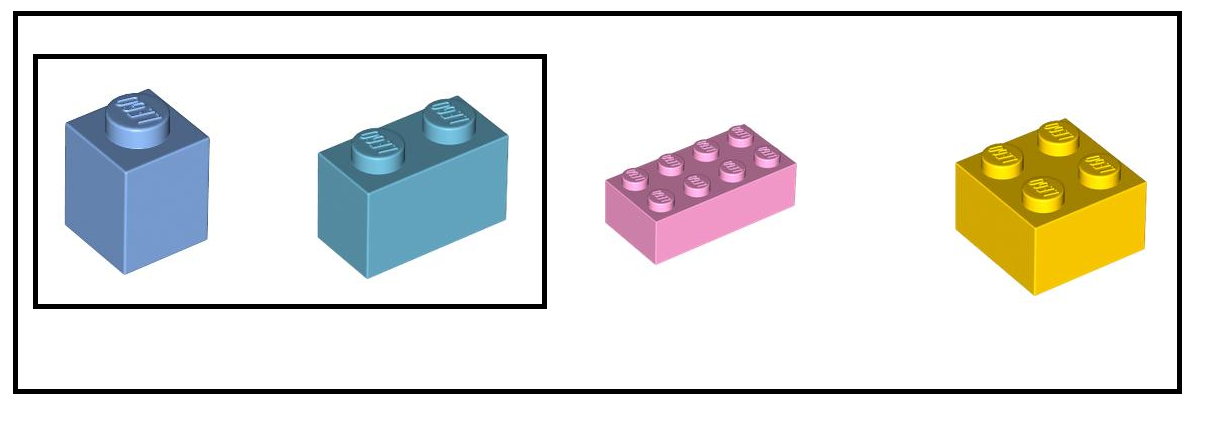
\includegraphics[width=0.6\columnwidth]{fig/scenario1_lego_set.png}
  \caption{LEGO Steintypen für die Innen- und Außenwände. (TODO Bild ist sehr hässlich)}
  \label{fig:Scenario1 Lego Set}
\end{figure}
Nicht nur die Abmessungen der Wände müssen in ein Raster fallen, auch deren Rotation wird in diesem Szenario auf 90\textdegree{} Schritte limitiert. 
Das stellt in diesem Fall eine vertretbare Enschränkung dar, da es ohnehin dem intuitiven Umgang mit LEGO Steinen und gleichzeitig dem Baustil der meisten einfachen Gebäuden entspricht.

\subsection*{Problemstellungen}
\begin{itemize}
  \item Wie können Öffnungen berücksichtigt werden?
  \item Stürze
  \item Verschiedene Wanddicken
  \item Übergänge zwischen verschiedenen Wanddicken
  \item T-Kreuzungen? Doch noch einbauen? Vlt die untere dünne wand dick machen?
\end{itemize}

\section{Scenario 3}\label{scenarios:scenario3}
Bauplandeduktion eines Gebäudemodells des KIT
\subsection*{Beschreibung}
Um das Konzept nicht nur an eigens modellierten Gebäuden zu evaluieren, werden zusätzlich externe Modelle herangezogen.
Dabei kann sich zum Beispiel an den Beispielprojekten des KIT bedient werden~\cite{KITSAMPLEHOUSE:online}.
TODO Bild von kleinem Hause
TODO überlegen ob eines der beiden riesendinger auch mal ran soll?
\subsection*{Problemstellungen}

\section{Scenario 4}\label{scenarios:scenario4}
Definition von Regelsets.
\subsection*{Beschreibung}
\subsection*{Problemstellungen}
\begin{itemize}
  \item Wie können Regelsets ohne Code vorgegeben werden? Also in welchem Format.
  \item In welcher Weise werden die Regeln dann angewendet etc?
\end{itemize}
\chapter{Problemstellung}\label{problem}
Ziel der Arbeit ist es einen Workflow zu schaffen, welcher es einem Nutzer ermöglicht ein Gebäude in einem 3D Designer zu planen, das im Anschluss in einen durch einen heterogenen Roboterschwarm ausführbaren Bauplan übersetzt wird.
Dies erfolgt in mehreren Schritten, welche sich jeweils mit unterschiedlichen Fragestellungen befassen.
Anhand der Teilschritte lässt sich diese umfangreiche Problemstellung logisch einteilen und die jeweilgen Kernprobleme und Fragestellungen der einzelnen Schritte werden klar.


Roboter auf Mauer -> Test nicht mit Schaumstoffbricks möglich da gewicht
Lücken (Fenster, Türen)

\section{Bausteindefinition}
Wie können wir zu einem bestimmten Wandtyp ein Set an Bausteintypen definieren, mit welchen Wände diesen Typs gebaut werden müssen.
Dabei sollen die Bausteine nicht auf Quader beschränkt, sondern beliebige Körpern sein können.
Ebenfalls relevant sind eventuelle die Bausteinverbindungen, die ebenfalls Einschränkungen haben.
Ein Beispiel dafür ist etwa Mörtel bei Ziegelwänden.

\section{Wall-Detailing und Tiling}
Wie kann man algorithmisch mit einem Set an Bausteintypen eine Wand, welche als Mesh vorliegt, vollständig erbauen und daraus einen Bauplan herleiten (Stichwort Abhängigkeitsgraph).

\section{Definition Bauplan}
Was muss ein Bauplan konkret beinhalten?
LALAB
\section{Aufgabenstellung}
Nachfolgend werden in chronologischer Reihenfolge alle notwendigen Teilaufgaben aufgezeigt, die gelöst werden müssen, um ein Gebäude zu planen, welches anschließend von Robotern gebaut werden kann.

\subsection{Modellierung des 3D Modells}
Es muss ein Weg gefunden werden, dem Nutzer das Modellieren von Teilstücken eines Gebäudes zu erleichtern, sodass er keine einzelnen Bauteile in dem Editor verwenden muss, sondern Konglomerate (wie etwa eine Wand oder ein Fenster) zur Verfügung hat, welche als Ganzes bewegt oder verformt werden können.
Dabei dürfen aber Informationen über die eigentlich zugrundeliegenden Bauteile (z.B. Ziegel) entweder nicht verloren gehen und implizit vorgegeben sein (z.B. durch das aufzwingen eines Rasters, welches dem Formfaktor der Bauteile entspricht, sodass etwa eine Wand nicht in beliebig kleinen Schritten vergrößert werden kann, sondern immer nur einen Längensprung um die Länge des kleinsten zugrundeliegenden Ziegel macht) oder das Programm versucht, das Gebäude nach beenden des Designprozesses möglichst gut mithilfe des vorgegebenen Sets an Bauteilen abzubilden. Das führt aber dazu einen möglichst guten Kompromiss finden zu müssen, was durch ein Raster von vornherein vermieden werden kann.

Fragestellung: Wie kann das Modellieren eines Gebäudes für Nutzer vereinfacht werden ohne wichtige Informationen zu verlieren?

\subsection{Finden eines geeigneten Dateiformats}
Wie breits vorweg genommen, muss es möglich sein aus dem Gebäudemodell eine Menge an Bauteilen von vorgegebenem Typen zu berechnen, die das Gebäude komplett (oder möglichst gut) abbildet.
Das geht entweder, indem man diese Menge während dem Designprozess impliziert vorliegen hat, da alle größeren Teilstücke (wie etwa eine Wand) schon mithilfe der zugrunde liegenden Bauteile definiert wurden oder durch das einmalige Konvertieren eines von den Bauteilen völlig losgelösten 3D Modells in eben jene Menge an Bauteilen.
Im ersten Fall fällt das Konvertieren weg und der Nutzer arbeitet immer direkt auf dem Datenformat, welches anschließend in späteren Schritten verwendet wird.
Im zweiten Fall kann das konvertierte Modell vermutlich nicht wieder in den Editor zurückgeladen werden, sodass man ein "Design Speicherformat" und ein "Konvertiertes Datenformat" hätte.
Dies ist aber ebenfalls eine gängige Praxis bei z.B. Vektorgraphik-Bearbeitungsprogrammen, die in einem proprietären Format Daten über mathematisch definierte Kurven halten und der Nutzer daraus Bilder in pixelbasierte Formaten wie jpg oder png generieren kann.
Dabei gehen viele Informationen verloren und man kann das exportierte Bild nicht in derselben Art wieder in das Programm laden.
Mit Blick auf die Domäne des Häuserbauens ist allerdings ein möglichst großer Freiheitsgrad wünschenswert, was für den Konvertierungsansatz spricht.
Dabei wird es wie bereits erwähnt herausfordernd eine möglichst gute Abbildung des im Editor designten Gebäudes mithilfe eines limitierten Sets an Bauteiltypen zu finden, welches nach Möglichkeit alle vom Nutzer gewünschten Eigenschaften behält.
Als Speicherformat kann ein im Bauingeneursbereich weit etablierter Standard verwendet werden, der neben den bloßen geometrischen Informationen über das Gebäude auch wichtige Details aus anderen Fachbereichen integriert.
Dieser Standard wird im weiteren Verlauf dieses Expos\'{e}s vorgestellt.

Fragestellung: Das Gebäude im Hintergrund immer als Menge von definierten Bauteilen oder als gängiges 3D Modell speichern, welches irgendwann in Bauteile überführt werden muss?

\subsection{Finden eines geeigneten Bauplans für Roboterschwärme}
Um dem Umfang und die Komplexität diesen Schrittes zu erfassen, wurde Ludwigs Dissertation gelesen \cite{Naegele2021}.
Diese beschäftigt sich mit dem Finden geeigneter Baupläne für beliebige Produkte mit Einbeziehung diverser (etwa geometrischer) Einschränkungen der Einzelteile oder der Monatageroboter.
Mit einem solchen Verfahren kann die derzeit teure Individualisierung von Produkten kosteneffizient ermöglicht werden, da sämtliche Produktionsschritte automatisch herausgefunden werden und damit Zeit sowohl in der Planung, als auch beim Einlernen der Montageroboter gespart werden kann.
Im Grunde ist die Problemstellung aus dieser Arbeit folgende:
Die Menge möglicher Baupläne für ein Produkt steigt exponentiell mit der Menge der verwendeten Bauteile und kann als sehr großer Suchraum für passende Lösungen angesehen werden, welcher z.B. mithilfe bestimmter Anforderungen an den resultierenden Bauplan verkleinert werden kann.
Tatsächlich kann diese Fragestellung direkt auf die Domäne des Häuserbauens angewendet werden:
Bei Gebäuden handelt es sich um Objekte mit vielen Tausend Bauteilen, was aufgrund des exponentiellen Wachstums des Suchraums zu einer unmöglich großen Menge potentieller Baupläne führt.
Um dem entgegenzuwirken, sucht man Constraints, wie etwa die Erkenntnis, dass Ziegel nur von unten nach oben aufgeschichtet werden können.
Damit fallen eine Vielzahl an Bauplänen weg und der Suchraum verkleinert sich erheblich.
Auch die Beschaffenheit der Bauteile und der Roboterendeffektoren und -körper bringen Constraints mit sich.
Allerdings ist der Einsatz von mehreren Robotern ein neuer Aspekt, der in Ludwigs Arbeit nicht berücksichtigt wird.
Dennoch liegt es nahe die Ergebnisse aus seiner Arbeit für dieses Projekt zu verwenden und für die Abarbeitung durch mehrere Agenten anzupassen.
Als Input für seinen "Suchalgorithums" wurde in Ludwigs Dissertation ein eigenes xml-artiges Datenformat zur vollständigen Beschreibung des fertigen Bauteils eingeführt auf Basis dessen ein nach einer Heuristik optimierter Bauplan herausgesucht wird.
Oftmals hat diese Heuristik zum Ziel, die Montagedauer oder die Kosten der Monatge zu minimieren.
Es ergibt Sinn dieses Format als Ergebnis aus dem vorherigen Schritt anzusehen.
Das bedeutet, dass das 3D Modell des Gebäudes in das von Ludwig verwendete Format übersetzt werden muss, welches alle für die Suchopertation notwendigen Informationen über die individuellen Bauteile besitzt.
Somit wird Ludiwgs Format zum "Konvertierten Datenformat", das aus dem 3D Modell berechnet wird.
Das Ergbnis der Suchoperation auf dem Konvertierten Datenformat stellt ein für einen heterogenen Roboterschwarm abarbeitbarer Bauplan dar.
Dafür muss die Suchoperation in Teilen angepasst werden.

Fragestellung: Wie wird aus dem Bauteilplan ein für Roboterschwärme abarbeitbarer Plan zur Erstellung des Gebäudes?

\subsection{Format zur Beschreibung der Bauteile aus welchen Wände bestehen}
Wie beschreibt man Bauteile, sodass neben der geometrischen Struktur z.B. auch die Berarbeitungsmöglichkeiten (wie etwa das Zerschneiden eines Ziegels) angegeben/eingeschränkt werden können.
Wie verwendet man diese Informationen, um Wände, die aus einem solchen Baustein errichtet werden sollen schon vorab im 3D Editor in die darin vorgegebenen Einschränlungen zu pressen (z.B. Legosteine sollten nicht zerschnitten werden -> es gibt also einen Stein, welcher als kleinste Größenänderung für die Wand gelten muss. Die Wand wird quasi in ein Grid gepresst. Wie sieht das aber aus, wenn es sich nicht um so einfache geometrische Körper handelt? -> sau rechenaufwendig?)
% https://academy.ifcopenshell.org/posts/using-ifcopenshell-and-pythonocc-to-generate-cross-sections-directly-from-an-ifc-file/
% https://blenderbim.org/docs-python/ifcopenshell-python/geometry_processing.html
%https://academy.ifcopenshell.org/posts/using-ifcopenshell-and-pythonocc-to-construct-new-geometry/

\chapter{Grundlagen}\label{basics}
Zunächst wird für diese Arbeit ein geeignetes Speicherformat für 3D Modelle von Gebäuden benötigt.
Um den Bau von Gebäuden zu automatisieren, ist es notwendig die Domäne \textit{Gebäude} möglichst vollständig digital abbilden zu können. 
Hilfreich ist dabei, wichtige Daten über bestimmte Bestandteile des Gebäudes direkt in das Modell zu integrieren, auf Basis derer etwa Kostenberechnungen durchgeführt oder Materialmengen herausgefunden werden können.
Da diese Informationen oft von Experten verschiedener Fachbereiche (etwa aus den Bereichen der Architektur, des Bauwesens oder der Statik) stammen, muss das Format sehr flexibel und im besten Fall auch zeitgleich bearbeitbar sein.
Dafür werden seit dem Jahr 2000 die \textit{Industry Foundation Classes} (IFC) von buildingsmart entwickelt, deren Anwendung im internationalen Bauwesen mittlerweile weit verbreitet ist~\cite{Industry61:online}.


\section{Industry Foundation Classes}\label{basics:ifc}
In der Spezifikation des Standards selbst, wird dieser wie folgt beschrieben:
\glqq{}Die Industry Foundation Classes (IFC) sind ein offener internationaler Standard für Daten des Building Information Model (BIM), welche zwischen Softwareanwendungen ausgetauscht, gemeinsam genutzt und von den verschiedenen Akteuren der Bauindustrie und des Gebäudemanagements verwendet werden. 
Der Standard enthält Definitionen für Daten, die für die Lebenszyklen von Gebäude- und Infrastrukturarbeiten erforderlich sind. 
Die bis jetzt in die IFC aufgenommenen Infrastrukturtypen umfassen Brücken, Straßen, Eisenbahnen, Wasserstraßen und Hafenanlagen\grqq{} (aus dem Englischen)~\cite{IFCScope:online}. 
Eine frühere Version des IFC Standards ist unter der Bezeichnung ISO 16739 registriert (siehe~\cite{ISOISO1694:online}).
Da die IFC aber nach wie vor kontinuierlich weiterentwickelt werden, wird in dieser Arbeit die derzeit neueste Version verwendet.
Diese ist die IFC Spezifikation 4.3.1.0~\cite{IFC4310Spezification:online}.
Das verbreitetste Austauschformat für IFC ist das Step Physical File Format, welches im ISO 10303 Teil 21 registriert ist~\cite{ISO_Step:online}.
Zudem gibt es speicherreduzierte Formate wie ifcZip oder für Menschen lesbarere Formate wie ifcXML~\cite{Industry93:online}\cite{IFCForma28:online}\cite{BIM_handbook_AEC_XML_SCHEMAS}.

\subsection{IFC 4.3.1.0 Aufbau}
Im Grunde definieren die \textit{Industry Foundation Classes} eine Vielzahl an Klassen, die in einer komplexen Hierarchie angeordnet den Grundstock des Datenmodells bilden.
Diese sind anfangs abstrakte Konzepte, die sich mit zunehmender Tiefe in der Hierarche konkretisieren.
\begin{figure}[ht]
    \centering
    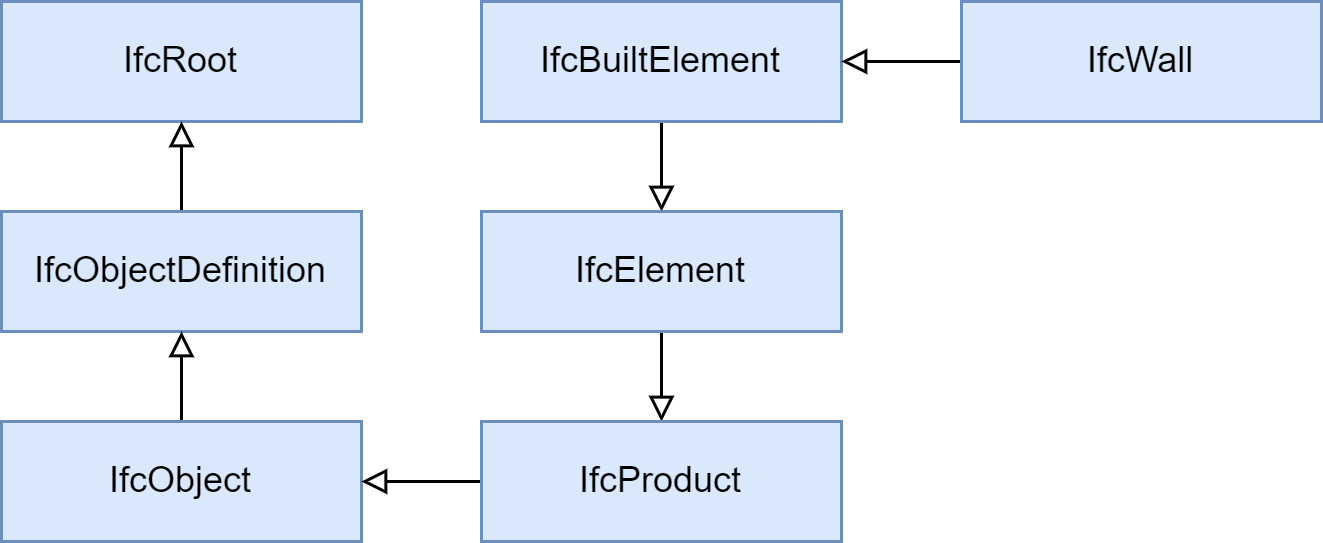
\includegraphics[width=0.6\columnwidth]{fig/Hierarchie_IfcWall_300.drawio.png}
    \caption{Klassenhierarchie am Beispiel der Klasse \textit{IfcWall}}
    \label{fig:IfcWall_Hierarchie}
\end{figure}
Da sich diese Arbeit zum größten Teil mit aus Wänden bestehenden Gebäuden befasst, wird nachfolgend die Klasse \textit{IfcWall} wiederholt als Beispiel herangezogen.
Der für diese Klasse relevante Ausschnitt aus der Klassenhierarchie ist in Abbildung~\ref{fig:IfcWall_Hierarchie} dargestellt.
Objekte werden von dem Standard in Relation zueinander gestellt, um komplexere Zusammenhänge darzustellen.
In Abbildung~\ref{fig:IFC_Relationships} erkennt man den Zusammenhang zwischen einem Objekt des Types \textit{IfcWall}, des Stockerwerks, welches diese Wand referenziert und wiederum selbst Teil eines \textit{IfcBuildings} ist, bis hin zur obersten Komponente eines Ifc Projektes, dem gleichnamigen \textit{IfcProject}.

\begin{figure}[h]
    \centering
    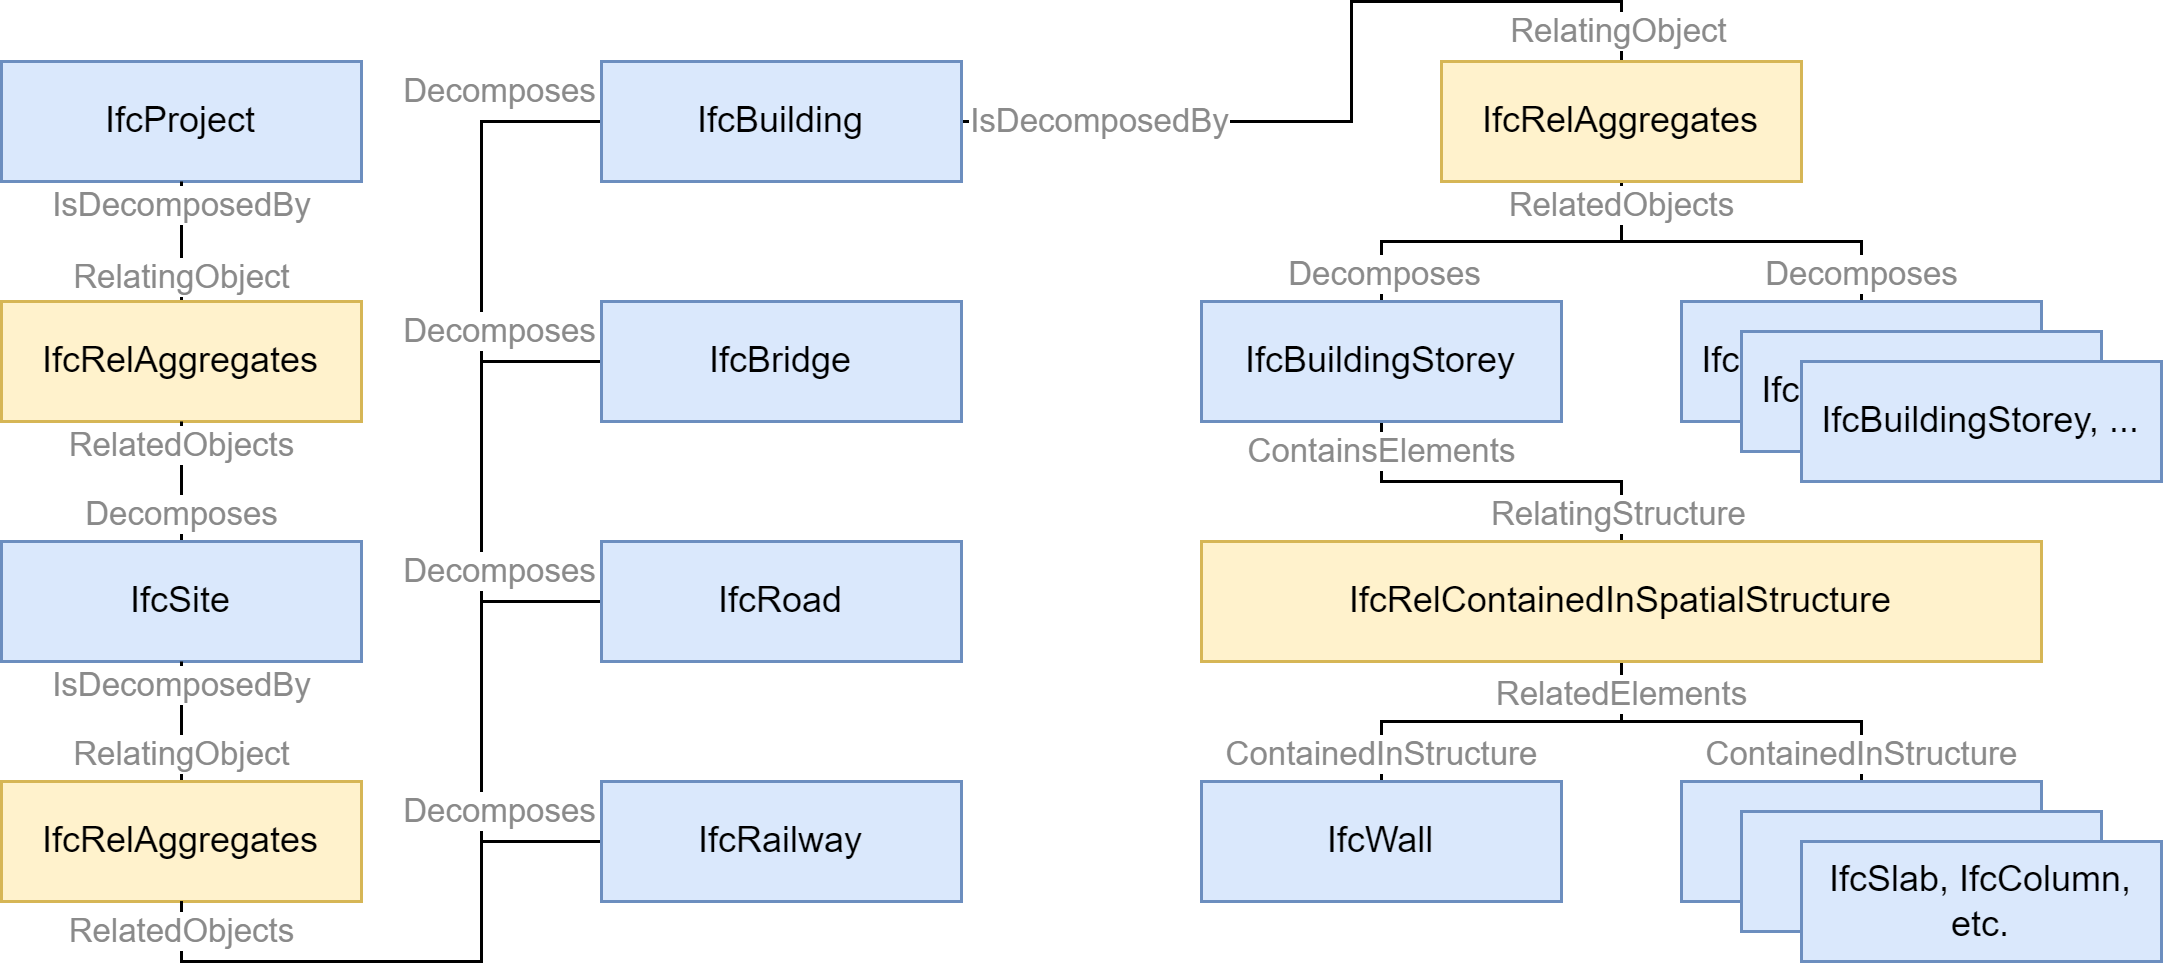
\includegraphics[width=0.9\columnwidth]{fig/IFC_Relationships_300.drawio.png}
    \caption{Relation der IfcWall und einem \textit{IfcProject}}
    \label{fig:IFC_Relationships}
\end{figure}

\subsection{IfcPropertySets und IfcQuantitySets}\label{basics:ifc_properties}
Mit dem Erweitern des Gebäudemodells um möglichst viele Informationen, schafft man einen detailierten digitalen Zwilling, der neben der bloßen Darstellung des Gebäudes als 3D Modell zusätzlich die Untersuchung auf andere Eigenschaften ermöglicht.
Dazu zählen zum Beispiel eine präzisere Kosten- und Zeitschätzung, Sicherheitsaspekte und Emissionen eines Bauvorhabens~\cite{Industry93:online}~\cite{Ding2014}. 
Dies ist mithilfe von \textit{IfcPropertySets} und \textit{IfcQuantitySets} umsetzbar, welche Objekten oder Objekttypen angehängt werden können.
Dabei werden IfcQuantitySets vorwiegend dazu verwendet numerische Werte zu geometrischen oder physikalischen Eigenschaften auszudrücken.
IfcPropertySets dienen hingegen dazu bestimmten Objekten oder Objekttypen mit sämtlichen nicht numerischen Werten zu annotieren.
Beispiele dafür sind etwa Material oder Farbe eines bestimmten Objekts.
Die Verwendung der Bezeichnung \textit{Set} rührt daher, dass diese Informationen in einer Baumstruktur vorliegen und demnach verschachtelt sein können.
Es gibt zu vielen Klassenbeschreibungen des IFC Standards vordefinierte PropertySets.
Das hilft dabei wichtige Informationen zu bestimmten Objekttypen einheitlich angeben zu können.
Im Falle des \textit{IfcWallType} existiert beispielsweise das PropertySet mit dem Namen \textit{Pset\_WallCommon}~\cite{IFC4310PSetWallCommon:online}.
Darin können die Ersteller von neuen WallTypes unter anderem Informationen über Brennbarkeit, thermisches Verhalten oder Akustik hinterlegen.
Bei Erstellen einer IfcWall-Instanz aus einem bestimmten WallType werden die damit verbundenen Property- und QuantitySets automatisch daran angehängt, sodass jedes Objekt relevante Informationen über sich selbst bereithält.

\subsection{Positionierung von \textit{IfcProducts}}
%https://ifc43-docs.standards.buildingsmart.org/IFC/RELEASE/IFC4x3/HTML/concepts/Product_Shape/Product_Placement/Product_Local_Placement/content.html
Die Platzierung eines \textit{IfcProducts} wird durch eine Verkettung relativer Transformationen ausgehend vom \textit{IfcProduct}, über sätmliche Strukturen, die dieses Objekt enthalten, bis hin zur \textit{IfcSite} realisiert~\cite{IFCPlatzierung}.
Diese Hierarche kann der Abbildung~\ref{fig:IFC_Relationships} entnommen werden.
Um die globale Position eines \textit{IfcProducts} zu erhalten, müssen die relativen Transformationen miteinander verrechnet werden.
Der IFC Standard unterstützt zudem die Möglichkeit Positionierungen anhand eines Rasters oder mithilfe des sogennanten \textit{linear placements} anzugeben.

\subsection{IfcOpeningElement}
\label{basics:IfcOpeningElement}
Neben Wänden stellen Fenster und Türen wichtige Elemente eines Gebäudes dar.
Diese sind ebenfalls Teil der Klassen des IFC Standards.
Objekte des Typs \textit{IfcOpeningElement} dienen dazu die notwendigen Lücken in einer Wand zu definieren in die später eine Tür oder ein Fenster eingebaut werden soll.
In der Dokumentation wird dies wie folgt formuliert (aus dem Englischen): \glqq{}[Das IfcOpeningElement] stellt eine Lücke in jedem Element dar, das eine physische Manifestation hat\grqq{}~\cite{IFC4310OpeningElement:online}.
Es gibt zwei Arten an IfcOpeningElement, je nachdem ob die Öffnung durch die gesamte Breite eines Objektes reicht oder nicht. 
Folglich entsteht dadurch eine Unterscheidung zwischen Nischen und tatsächlichen Öffnungen, wobei nur letztere im Zusammenhang mit Fenstern oder Türen Sinn ergibt.
TODO: Diagramm zwischen IFCWall und IfcOpeningElement.

\section{IFC for Blender}\label{basics:blender}
\subsection{Blender}
Blender ist eines der beliebtesten Open Source Programme zur Modellierung von 3D Modellen und Animationen~\cite{blendero56:online}.
Eine umfangreiche Python API erlaubt es Blender durch sogenannte Addons an die eigenen Bedürfnisse anzupassen~\cite{PythonWebsite:online}~\cite{BlenderPythonAPI:online}.
Aufgrund dessen existiert auch eine Vielzahl an freien Erweiterungen \textendash{} unter anderem auch eine Integration von IFC Projekten.

\subsection{blenderbim}
Neben kommerziellen Produkten wie etwa revit von autodesk zur Modellierung von IFC Modellen, gibt es auch für Blender ein freies Plugin, um IFC Modelle zu erstellen~\cite{RevitSof26:online}~\cite{BlenderB43:online}.
Dieses Plugin ermöglicht es neben dem bloßen Designen des Gebäudes in kurzer Zeit z.B. detailierte Zeichnungen verschiedener Perspektiven herauszuarbeiten, die z.B. von Bauingeneuren verwendet werden können, um einzelne Stockwerke oder Verkabelungen zu planen.
Blenderbim selbst kapselt unter anderem die Open Source Python Bibliothek \textit{IfcOpenShell}, sodass diese in der Blender Laufzeitumgebung zur Verfügung steht \cite{IFCOpenShell:online}.

\subsection{IfcOpenShell}\label{basics:ifcopenshell}
\begin{lstlisting}[label={basics:ifcopenshell_sample_code}, language=Python, caption=Beispielprogramm zur Extraktion bestimmter Daten einer IFC Datei und Generierung eines Meshes aus deren geometrischen Representationen.]
import ifcopenshell
from ifcopenshell import geom
from stl import mesh, Mode
import numpy as np

settings = ifcopenshell.geom.settings()
settings.set(settings.USE_WORLD_COORDS, True)

ifc_file = ifcopenshell.open("model.ifc")
products = ifc_file.by_type("IfcProduct")
meshes = []

for product in products:
    if product.Representation and product.is_a("IfcWall"):
        shape = ifcopenshell.geom.create_shape(settings, product)
        vertices = np.array(shape.geometry.verts).reshape((-1, 3))
        edges = np.array(shape.geometry.edges)
        faces = np.array(shape.geometry.faces).reshape((-1, 3))

        m = mesh.Mesh(np.zeros(faces.shape[0], dtype=mesh.Mesh.dtype))
        for i, f in enumerate(faces):
            for j in range(3):
                m.vectors[i][j] = vertices[f[j], :]
        meshes.append(m)

# Create the combined mesh
combined = mesh.Mesh(np.concatenate([m.data for m in meshes]))
combined.save('model.stl', mode=Mode.ASCII)
\end{lstlisting}

IfcOpenShell ist eine frei verfügbare Bibliothek, die es erleichtert mit Daten im IFC Format zu arbeiten.
Sie bietet unter anderem eine Python API an und ist wie bereits erwähnt ein Teil des Blender Addons blenderbim.
Natürlich ist es dennoch möglich diese Bibliothek auch ohne Blender zu verwenden.
In Listing~\ref{basics:ifcopenshell_sample_code} ist ein kurzes Beispiel eines Programmes gegeben, das in einer IFC Datei alle Objekte des Typs IfcWall ausfindig macht und dessen geometrische Representation in ein herkömmliches Mesh konvertiert.
Damit existiert ein intuitiver Zugang zu den Daten von IFC Dateien.

\section{Building Information Modeling}\label{basics:bim}
Ein weiterer Punkt, der für die Verwendung von IFC spricht ist das sogenannte \textit{Building Information Modeling} (BIM)~\cite{Building41:online}.
Ein Definitionsvorschlag lautet wie folgt: \glqq{}BIM ist definiert als der Einsatz von Informations- und Kommunikationstechnologien zur Verschlankung der Prozesse im Lebenszyklus von Gebäuden, um eine sicherere und produktivere Umgebung für die Bewohner zu schaffen, die Umwelt so wenig wie möglich zu belasten und die Effizienz der Betriebsabläufe für die Eigentümer während des gesamten Lebenszyklus des Gebäudes zu erhöhen\grqq{} (Übersetzt aus dem Englischen)~\cite{Microsof51:online}.
Zum Lebenszyklus eines Gebäudes gehören etwa anfangs das Planen und Designen, später das Bauen, das Verwenden und Instandhalten und nach eventuellen Renovierungen das Abreißen.
BIM kommt in all diesen Phasen zum Tragen und erleichtert diese Prozesse durch Anbieten einer einheitlichen Schnittstelle für alle am Infrastrukturbau und -management beteiligten Personen.
Zusätzlich ermöglicht BIM eine exakte Dokumentation des Geschehens in sämtlichen Phasen des Bauwerks, was unter anderem zu einer genaueren Zeit- und Kostenplanung führt~\cite{Ding2014}.
Auch Verantwortlichkeiten sind Teil von BIM, was zu einer erhöhten Produktivität beiträgt.
Um nun das Zusammenarbeiten der unterschiedlichen Fachbereiche zu erleichtern, gibt es sogennante BIM-Server auf welchen mehrere Arbeitende synchron an einem Projekt arbeiten können, während sie jeweils die für ihren Aufgabenbereich passende Ansicht vor sich haben.
BIM-Server unterstützen zusätzlich eine Versionierung des Fortschritts an einem Projekt.

In einem Gespräch mit einem Ingeneur aus dem Bereich \glqq{}Energysystemtechnik\grqq{} kam zur Sprache, dass viele Bereiche von BIM noch nicht ganz Einzug in Deutschland gefunden haben.
Eben jene \glqq{}Kollaboration über einen BIM-Server mit Änderungsmanagement etc. [sei] (noch) nicht üblich, da noch nicht alle Beteiligten dazu in der Lage sind. Vor allem Bauherren, Architekten und Baufirmen können es nicht\grqq{}.
Weiter sei \glqq{}auch unklar, wer für falsche Angaben haftet und wer die Konsistenz aller Daten gewährleistet\grqq{}.
Auf der anderen Seite sei \glqq{}das im BIM festegelegte Datenformat IFC das Maß der Dinge und auch bei uns so in Verwendung\grqq{}.
Auch das Einpflegen \glqq{}ergänzende[r] Bauteilinformationen (z.B. zu Gewicht, Dämmwert, Recyclebarkeit, CO2 Fußabdruck, etc.)\grqq{} finden Einsatz und sind Teil seines Alltags.
Für ihn wichtig ist ebenfalls der Betrieb des Gebäudes.
Hier unterstützt BIM, indem sämtliche Teile der Installationen in einem Gebäude, wie z.B Fensterdichtungen, Kabel, Rohre, Sicherungen oder eine Umwälzpumpe individuelle Teilenummern zugewiesen bekommen, hinter welchen alle Daten wie etwa Hersteller, Bestellnummern, Lebensdauer, Wartungshistorie oder Entsorgungsnachweise vermerkt sind.
Dies wurde allerdings \glqq{}angesichts der Realität der Handwerker und Gebäudenutzer für völlig unrealisitsch und auch etwas over-engineered\grqq{} eingestuft.
Trotzdem sei \glqq{}BIM [\ldots] das große Ding in der Bauwelt und der einzige echte Standard\grqq{}.

\section{opensourcebim}
Während es vorwiegend kommerzielle Produkte gibt, die Unternehmen das Arbeiten mit BIM ermöglichen, exisitiert auch hier eine aktive Open Source Bewegung.
Unter dem Namem \glqq{}The open source BIM collective\grqq{} oder kurz \glqq{}opensourceBIM\grqq{} werden derzeit um die 70 Repositories betrieben.
Darin enthalten sind unter anderem ein BIM-Server inklusive verschiedener Clients für Endanwender auf unterschiedlichen Systemen und Werkzeuge, die es erleichtern den IFC Files zu arbeiten~\cite{Theopens96:online}.
Ein kurzer Test hat gezeigt, dass die in Blender modellierte IFC Files tatsächlich über einen \glqq{}Anzeige-Client\grqq{}, der mit einem lokal gehosteten BIM-Server verbunden ist, angezeigt werden können.
Obwohl die Verwendung des BIM-Servers für diese Arbeit nicht notwendig ist, besteht die Option diesen künftig mit in den Workflow zu integrieren, da damit auch das simultante Arbeiten an einem IFC File möglich ist, was in Blender nur teilweise und mit dem Einsatz von Plugins ermöglicht wird.
Das stellt einen Praxisbezug zum aktuell verwendeten Stand dieser Technologien her, was in der oftmals konzeptionellen Natur der Forschung nicht immer der Fall ist.
Wie auch Blender untertützt BIM-Server das Einbinden von eigenen Plugins, sodass eine Erweiterung um neue Funktionalität möglich ist.
Die Plugins werden in Java geschrieben.
Der Server bietet aber auch eine REST Schnittstelle an, um Clients in anderen Sprachen anzubinden.

\section{Mauerwerksbau}
\label{basics: Mauerwerksbau}
Der Mauerwerksbau ist eine Art des Massivbaus, bei welchem Natur- oder Formsteine aufgeschichtet werden, um Wände beziehungsweise Mauern zu errichten.
Eine derart erbaute Wand besteht demnach aus (Bau)-Steinen und den dazwischen entstehenden Fugen.
Mörtel ist dabei nicht zwangsläufig notwendig.
Man spricht von trocken versetzten Steinen oder einer Trockenmauer, wenn darauf verzichtet wird.
Heutzutage wird fast ausschließlich mit quaderförmigen Formsteinen gebaut.
Zur Beschreibung solcher Formsteine existieren zwei relevante Größen.
Die eine ist das sogenannte \textit{Baunennmaß}, mit dem die tatsächliche Größe des Steins angegeben wird.
Die andere das \textit{Baurichtmaß}, das sich aus Baunennmaß und dem Fugenmaß zusammensetzt.

\subsection{Maßsysteme}
Als Maßsystem bezeichnet man das Vorgeben der Größen von Bausteinen anhand eines konkret definierten (Grund-)Moduls.
Zwei in Deutschland populäre Grundmodule sind zum einem das \textit{ISO-2848-Basismodul} mit Länge 100mm und zum anderen der Achtelmeter, verankert in der \textit{DIN 4172 Maßordnung im Hochbau}~\cite{ISO2848}\cite{DIN417224}.
Letzteres bezeichnet man daher auch als das oktametrische Maßsystem.
Nachfolgend wird auf dieses Maßsystem näher eingegangen.

\subsubsection*{Oktametrisches Maßsystem}
Baurichtmaße sind gemäß dem oktametrischen Maßsystem immer ein Vielfaches von \(12,5 cm\) (das entspricht \(1/8 m\)) und nach der Norm aber mindestens \(6.25cm\).
Dies gilt sowohl für Länge und Breite als auch für die Höhe der Steine.
Das System ist in der \textit{DIN 4172 Maßordnung im Hochbau} geregelt und ist ein fest definiertes Grundmaß für das Bauwesen in Europa~\cite{DIN417224}.
\begin{figure}[ht]
    \centering
    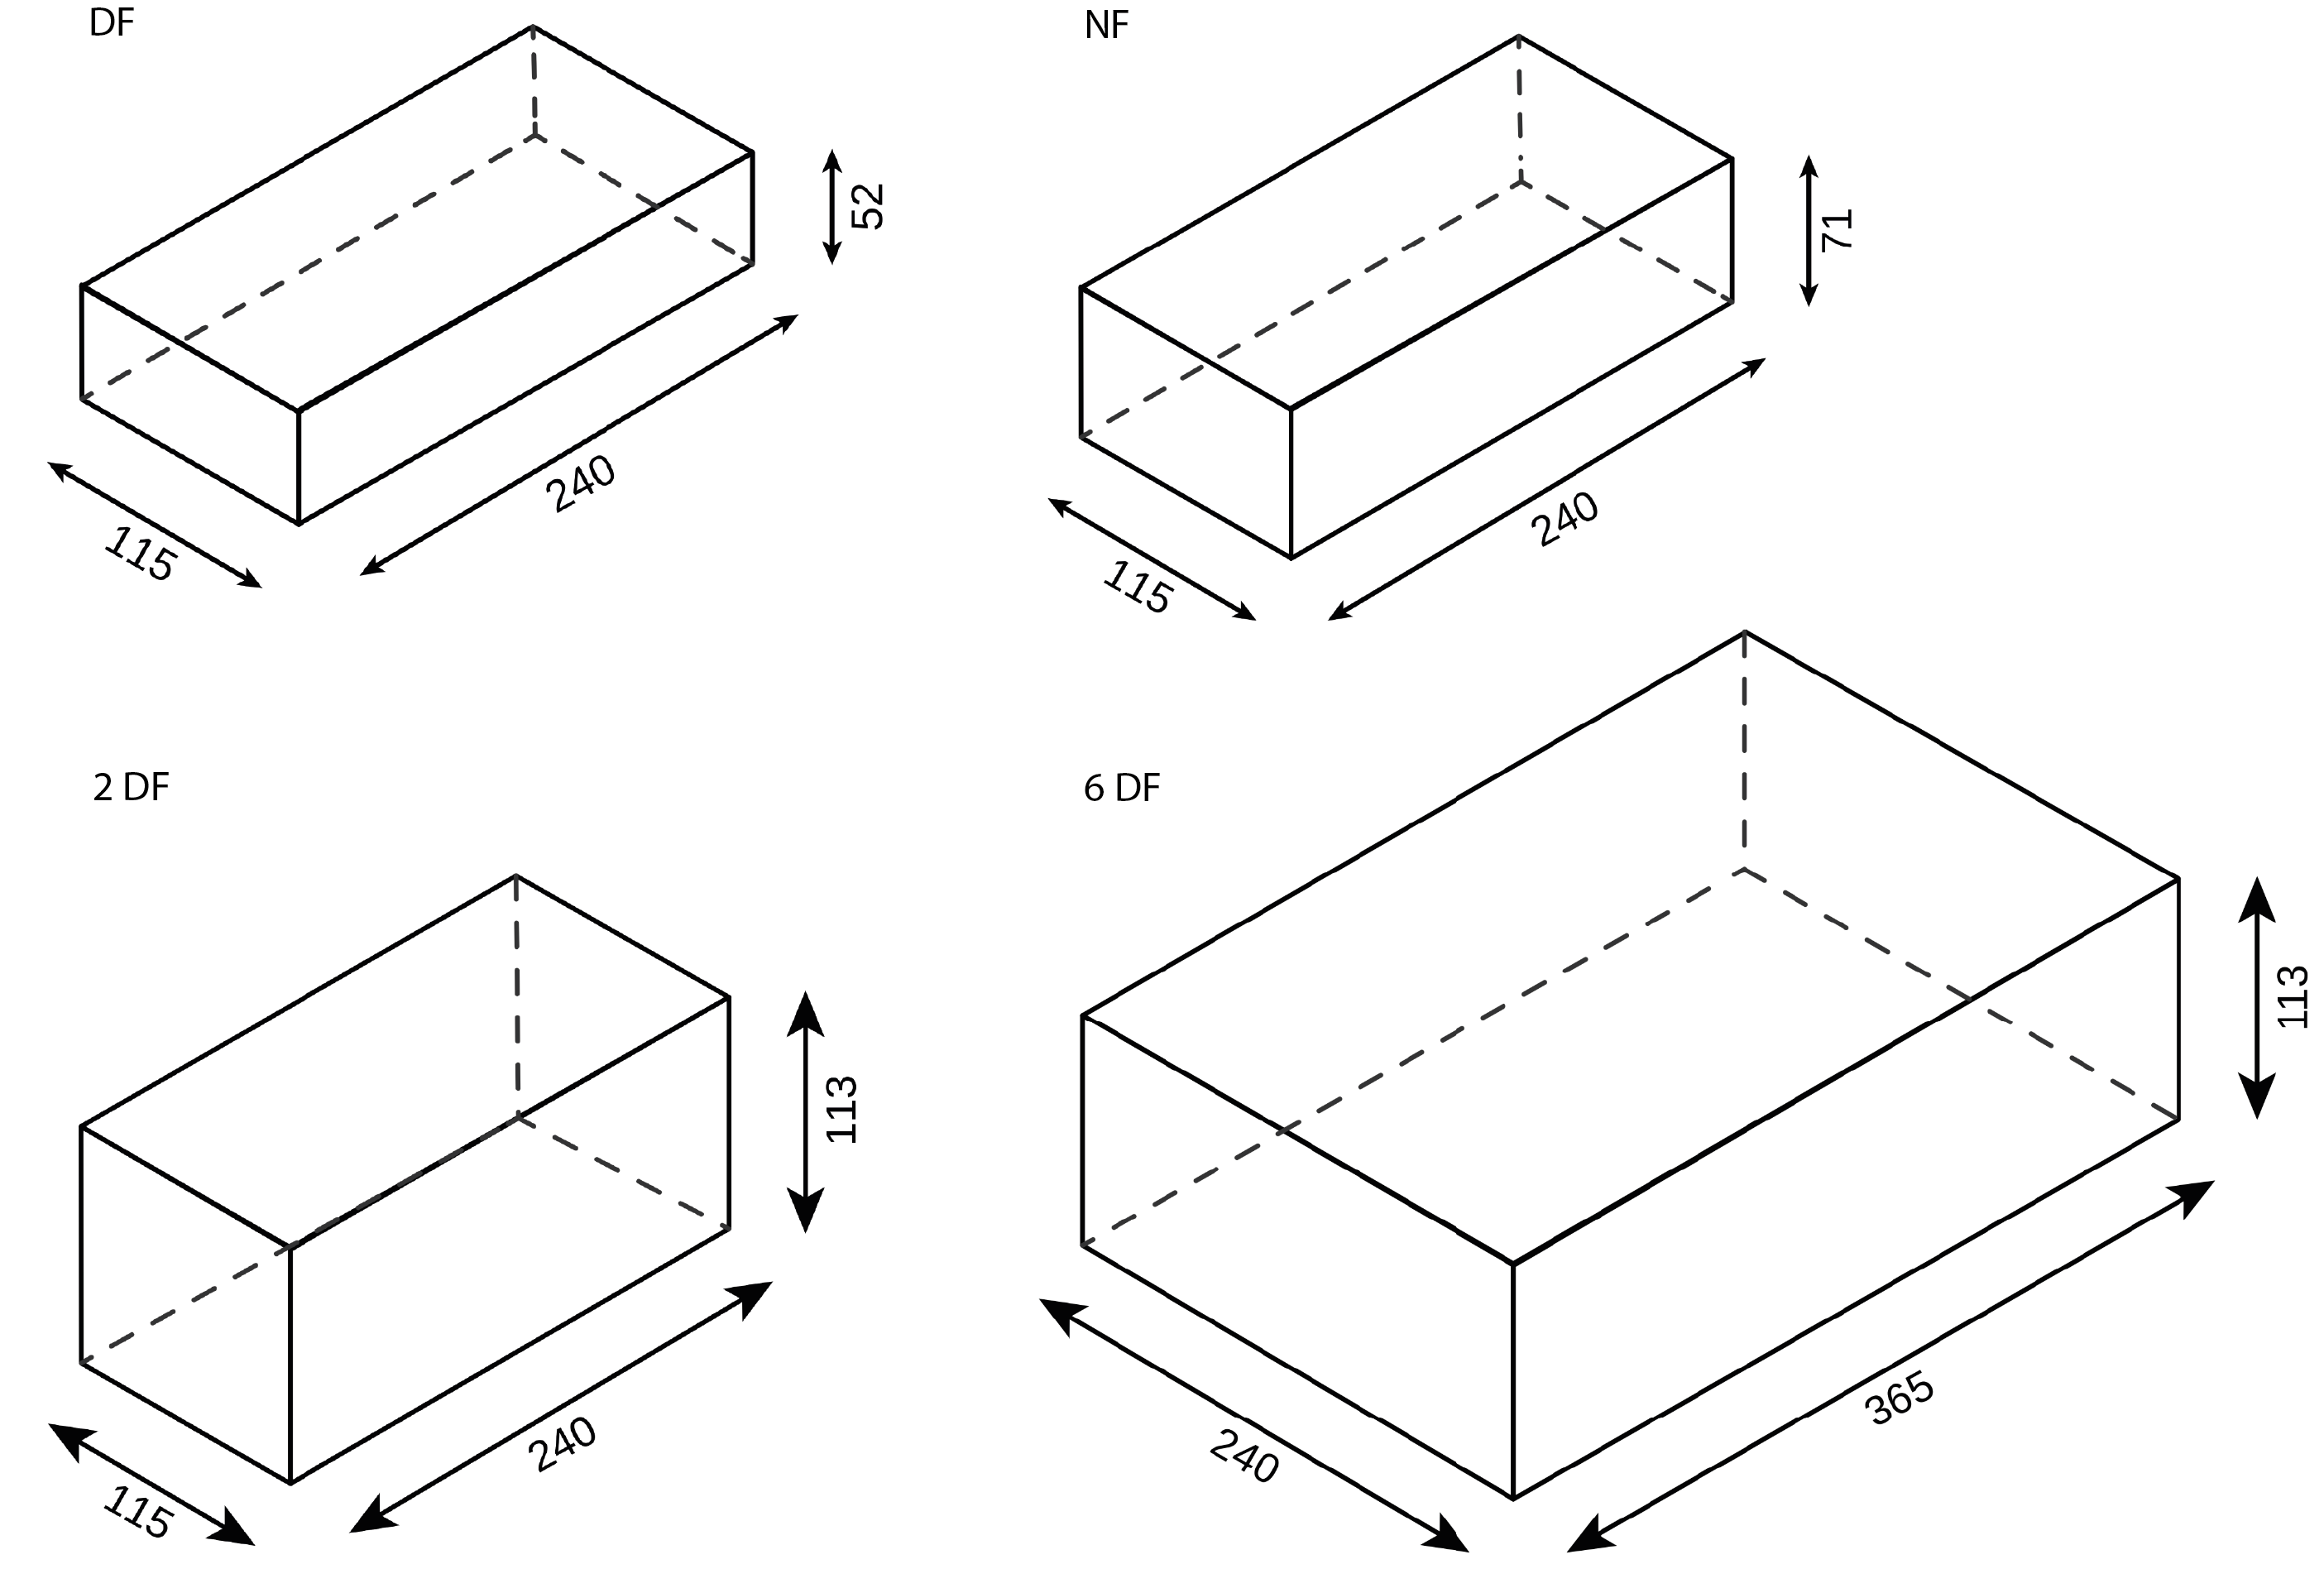
\includegraphics[width=0.8\columnwidth]{fig/Ziegelsteinformate DF NF 2DF 6DF.png}
    \caption{Darstellung verschiedener Steinformate nach DIN 4172 (Baunennmaß in Millimetern)~\cite{Steinfor38:online}}
    \label{fig:basics:Steinformate}
\end{figure}
\begin{figure}[hb]
  \centering
  \includegraphics[width=0.8\columnwidth]{fig/Oktametrische Maßordnung.png}
  \caption{Besondere Eigenschaften der oktametrischen Maßordnung~\cite{Moro2021}}
  \label{fig:basics:OktametrischeMassordnung}
\end{figure}
Daraus gehen insbesondere folgende zwei Formate für Ziegelsteine hervor:
Das Normalformat (NF) mit \(240\times115\times71 mm\) und das Dünnformat (DF) mit \(240\times115\times52 mm\) (Länge$\times$Breite$\times$Höhe)~\cite{Moro2021}.
Alle anderen Formate werden mithilfe dieser beiden Grundsteine angegeben.
So sind zum Beispiel die in Abbildung~\ref{fig:basics:Steinformate} gezeigten 2 DF und 6 DF Steine eine Kombination aus mehreren Steinen im Dünnformat.
Dabei sieht die Norm ein Fugenmaß von \(10 mm\) für Stoßfugen (vertikal) und \(12 mm\) for Lagerfugen (horizontal) vor.
Für Systeme, die eine schmalere oder keine Fuge benötigen, werden entsprechend größere Steine hergestellt, um der Maßordnung weiterhin zu entsprechen.
Durch Einhalten eines Systems ist man zusätzlich in der Lage Türen und Fenster an die daraus entstehenden Öffnungsgrößen anzupassen und vermeidet dadurch zeitaufwendiges, nachträgliches Anpassen.
Da Höhe, Breite und Länge der Steine zusammen mit den dazwischenliegenden Fugen aufgrund des Maßsystems jeweils Vielfache voneinander sind, ergeben sich viele Möglichkeiten zur Aufschichtung und Aneinanderreihung der Bausteine.
Einige davon sind in Abbildung~\ref{fig:basics:OktametrischeMassordnung} zu sehen und sind gleichzeitig Beispiele für einen sogenannten \textit{Mauerwerksverband}.

\subsection{Mauerwerksverband}
\label{basics:Mauerwerksverband}
Als Mauerwerksverband bezeichnet man bestimmte, gleichmäßige Anordnungen von Mauersteinen, um einen homogenen Mauerwerkskörper zu erreichen~\cite{Mauerwer39:online}.
Damit kann eine gleichmäßige Kraftverteilung innerhalb der Mauer gewährleistet werden.
Eine wichtige Rolle nimmt dabei das Überbindemaß ein, welches die Mindestüberlappung von Mauersteinen aus zwei Schichten der Mauer vorgibt.
Für das planmäßige Überbindemaß \(l_{ol}\) gilt für übliche Mauersteine mit Schichthöhen 
\(h_{u} \leq 249 mm\) 
nach DIN EN 1996-1-1: 
\(l_{ol} \geq 0,4h_{u} \geq 45 mm\)
~\cite{Bemessun72:online}\cite{DIN_EN_1996_1_1}.
Zudem wird darin die Mindestwanddicke für tragendes Mauerwerk, \glqq{}sofern aus Gründen der Standsicherheit, der Bauphysik oder des Brandschutzes nicht größere Dicken erforderlich sind\grqq{}~\cite{Bemessun72:online}, auf 
\(t_{min} = 115 mm\) 
festgelegt~\cite{DIN_EN_1996_1_1}.
Dies ist, wie in Abbildung~\ref{fig:basics:Steinformate} zu sehen, exakt die Breite der kleinsten Ziegelformate NF und DF.
Man unterscheidet zwei Arten von Mauerwerk: das Einsteinmauerwerk und das Verbandsmauerwerk.
Wie schon dem Namen zu entnehmen, handelt es sich beim Einsteinmauerwerk und ein Mauerwerk, bei welchem die Wanddicke der Steindicke entspricht.
Hier muss das Überbindemaß lediglich über die Wandlängsrichtung eingehalten werden.
Bei Verbandsmauerwerk gilt dies zusätzlich für die Wandquerrichtung~\cite{05maurer1:online}.
Einige Beispiele sind in Abbildung~\ref{fig:basics:verbaende} zu sehen.
\begin{figure}[htb]
  \begin{subfigure}[b]{0.5\columnwidth}
    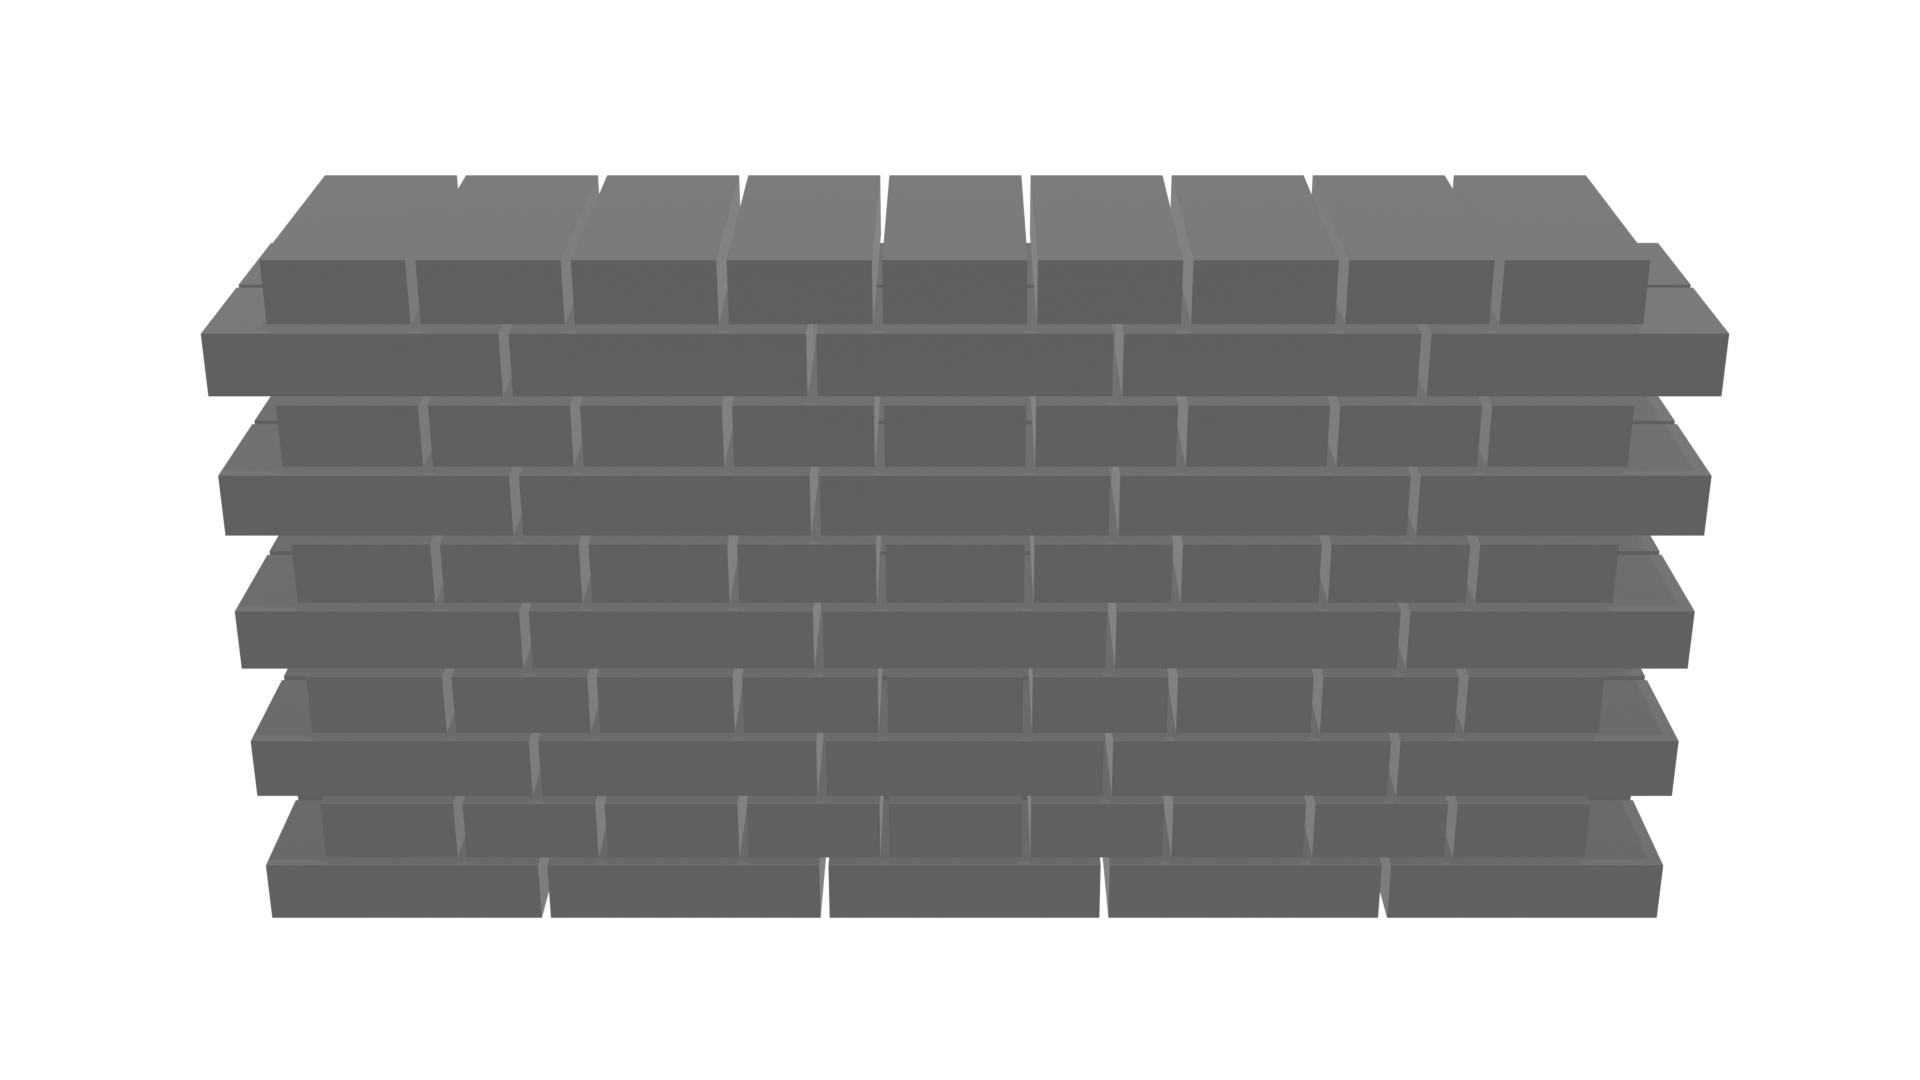
\includegraphics[width=\columnwidth]{fig/blockverband.png}
    \caption{Blockverband.}
    \label{fig:basics:blockverband}
  \end{subfigure}
  \hfill
  \begin{subfigure}[b]{0.5\columnwidth}
    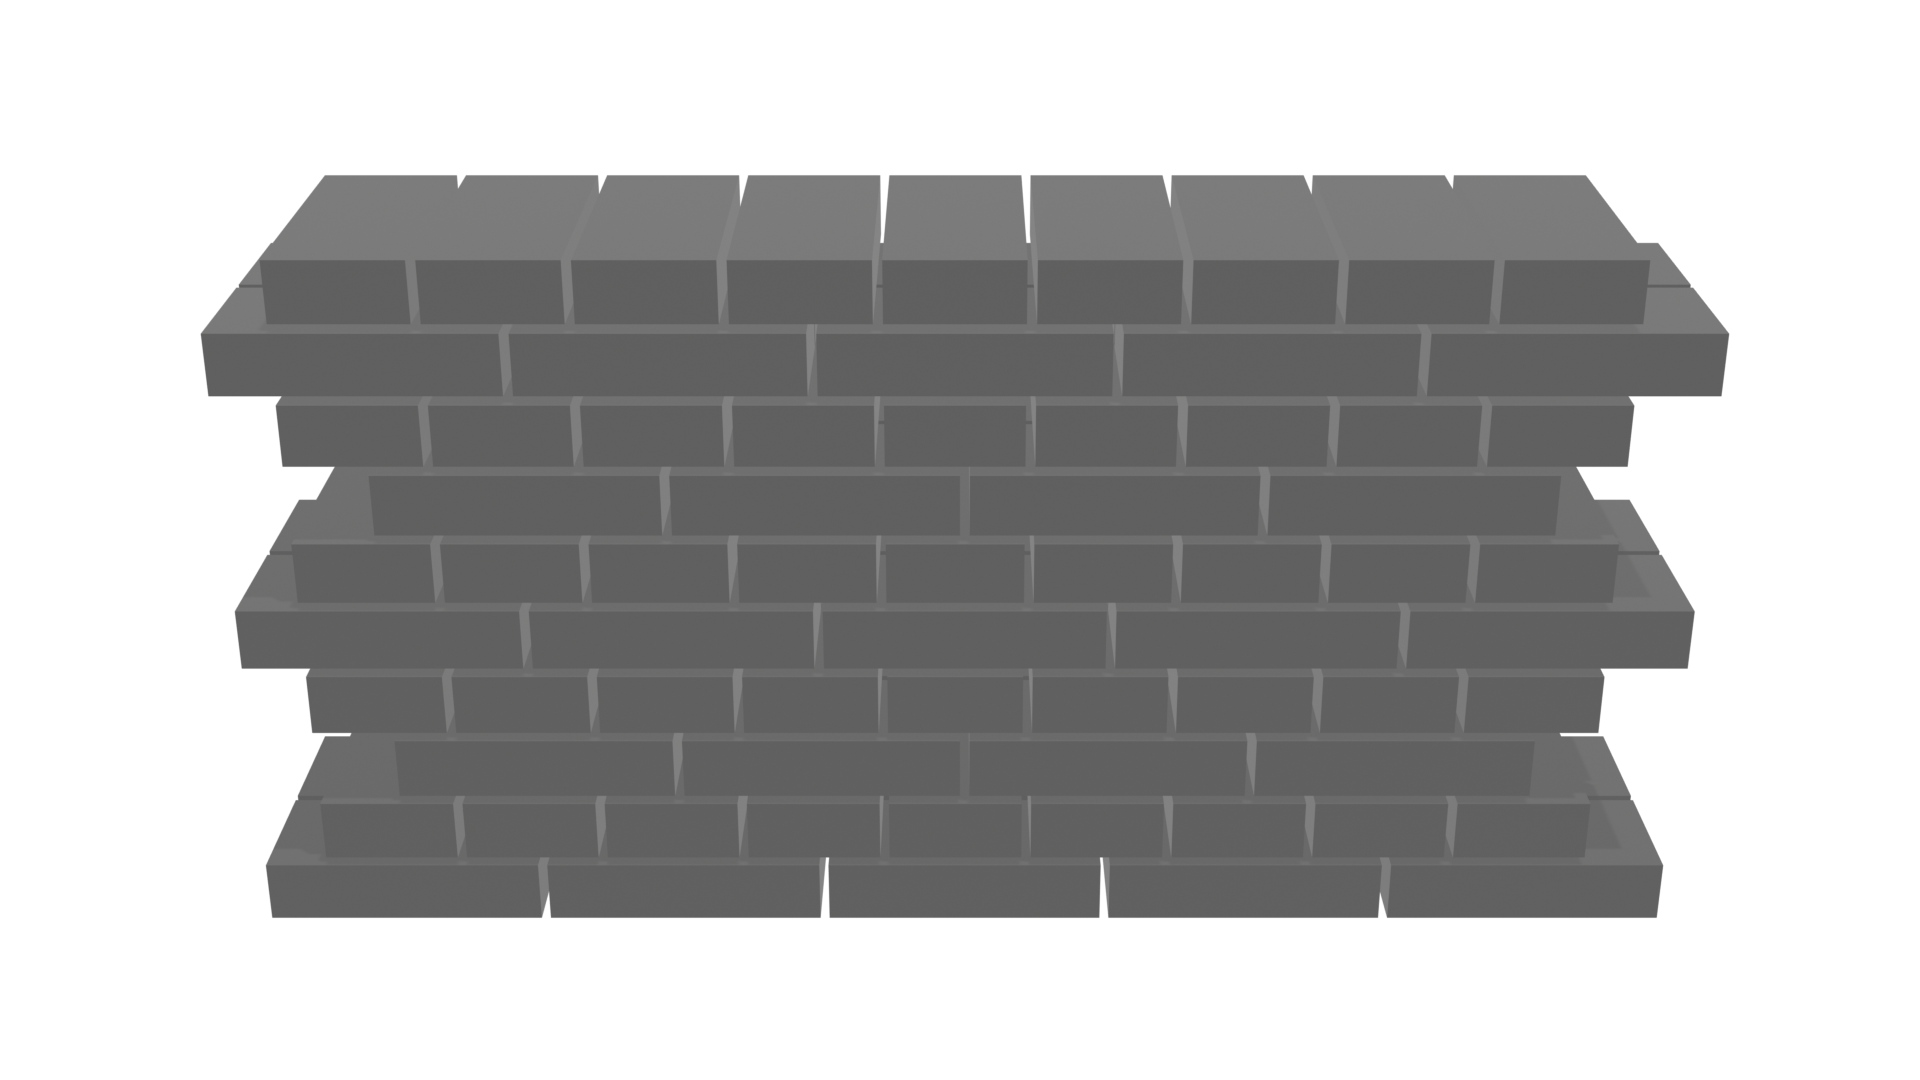
\includegraphics[width=\columnwidth]{fig/kreuzverband.png}
    \caption{Kreuzverband.}
    \label{fig:basics:kreuzverband}
  \end{subfigure}
  \begin{subfigure}[b]{0.5\columnwidth}
    \includegraphics[width=\columnwidth]{fig/läuferverband025_mittig.png}
    \caption{Mittlerer Läuferverband \textit{(1/4 Versatz).}}
    \label{fig:basics:laeuferverband_mittig}
  \end{subfigure}
  \begin{subfigure}[b]{0.5\columnwidth}
    \includegraphics[width=\columnwidth]{fig/läuferverband033_schleppend.png}
    \caption{Schleppender Läuferverband \textit{(1/3 Versatz).}}
    \label{fig:basics:laeuferverband_schleppend}
  \end{subfigure}
  \begin{subfigure}[b]{0.5\columnwidth}
    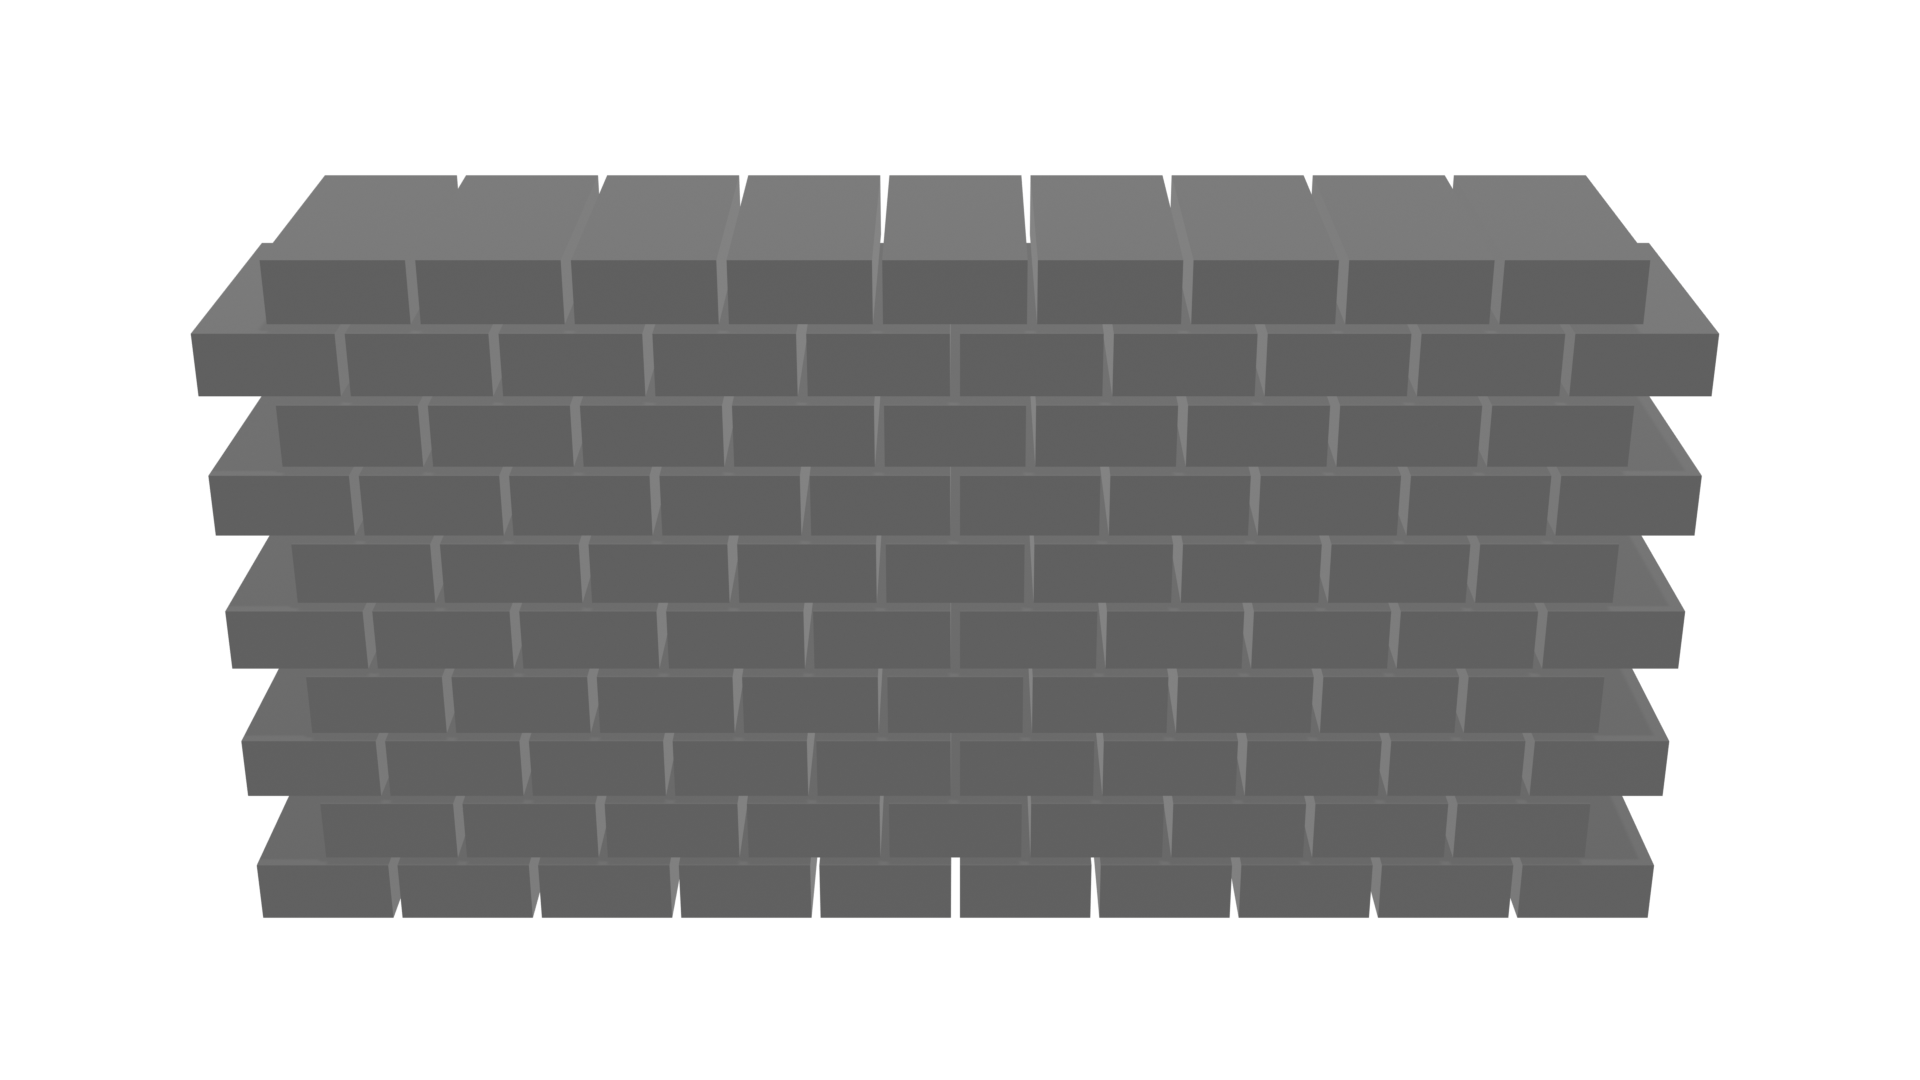
\includegraphics[width=\columnwidth]{fig/kopfverband.png}
    \caption{Kopf/Binderverband.}
    \label{fig:basics:binderverband}
  \end{subfigure}
  \begin{subfigure}[b]{0.5\columnwidth}
    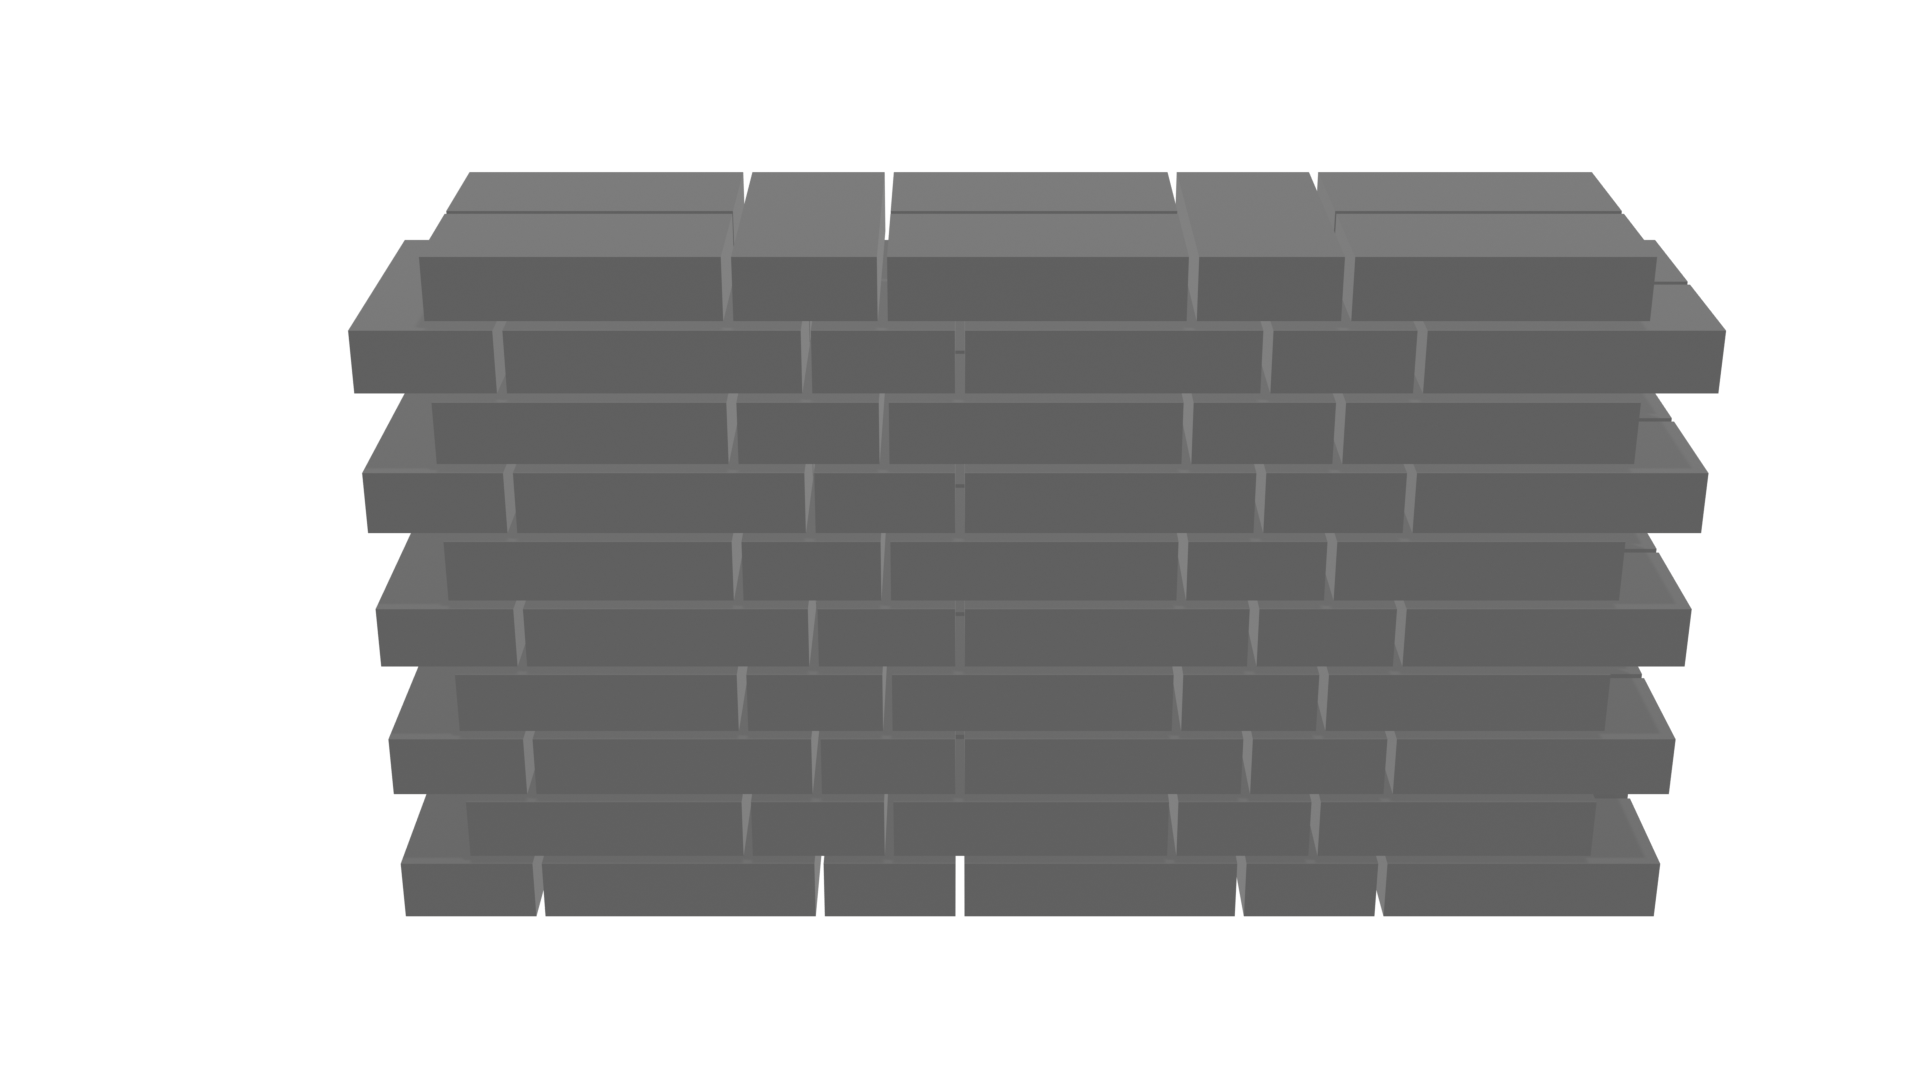
\includegraphics[width=\columnwidth]{fig/gotischerverband.png}
    \caption{Gotischer Verband.}
    \label{fig:basics:gotischer_verband}
  \end{subfigure}
  \caption{Typische Mauerwerksverbände.}
  \label{fig:basics:verbaende}
\end{figure}
Als Wandstück wird von nun an ein gerader Wandabschnitt bezeichnet.
Dieser hat eine Länge, eine Höhe und durch einen vorgegebenen Bausteintyp und einem gewünschten Verband eine gewisse Breite.
Treffen zwei oder mehrere Wandstücke aufeinander, so gilt es diese dem Überbindemaß entsprechend miteinander zu verzahnen.
Dabei treten verschiedene Sonderfälle auf, die für unterschiedliche Verbände nach unterschiedlichen Lösungen verlangen:
\begin{itemize}
  \item \textbf{Ecken} werden durch zwei sich an Wandenden berührenden, meist rechtwinklig zueinanderstehenden Wandstücken gebildet.
  \item \textbf{Kreuzungen} stellen zum Beispiel zwei sich kreuzende Wandstücke dar.
  \item \textbf{T-Kreuzungen} entstehen, wenn ein Wandende des einen Wandstücks auf einer anderen Wand steht.
  Sowohl bei Kreuzungen als auch T-Kreuzungen kann auf das aufwendige Verahnen verzichtet und stattdessen die sogenannte Stumpfstoßtechnik angewandt werden.
  Dabei werden Stahlanker zwischen der Wand und den darauf treffenden \glqq{}stumpfen\grqq{} Wandenden verwendet, um die beiden Wände sicher miteinander zu verbinden.
  \item \textbf{Wandenden} sind die \glqq{}Enden\grqq{} eines Wandstücks, die kein anderes Wandstück berühren.
  Dafür muss der verwendete Mauerwerksverband zu einem geraden Abschluss gebracht werden.
  Oftmals lässt sich das Anpassen der Bausteine (etwa durch zerschneiden) nicht vermeiden.
  \item \textbf{Öffnungen} innerhalb eines Wandstücks können in der selben Art behandelt werden, da der vorherrschende Verband in den betroffenen Schichten gerade unterbrochen werden muss.
  Über Öffnungen für Fenster und Türen wird ein sogenannter Sturz gelegt, welcher ebenfalls in den der Wand zugrunde liegenden Mauerwerksverband eingebunden werden muss.  
\end{itemize}
Die Lösungen für die oben geannten Situationen variieren je nach angestrebten Mauerwerksverband und der verwendeten Modulgröße stark.
Einige Beispiele sind in Abbildung~\ref{fig:basics:mauerwerk_eckloesung} und Abbildung~\ref{fig:basics:Kreuzungsloesung} zu sehen~\cite{Moro2021}\cite{MaurerfibelKreuzungen:online}.
Während etwa beim Läuferverband darauf verzichtet werden kann Bausteine für Eckbereiche und Kreuzungen zu zerschneiden, ist dies für andere Verbände teilweise unumgänglich. 

\begin{figure}[h]
  \centering
  \includegraphics[width=0.8\columnwidth]{fig/Eck- und Kreuzungslösungen.png}
  \caption{Lösungen für Ecken und T-Kreuzungen unterschiedlicher Verbände~\cite{Moro2021}}
  \label{fig:basics:mauerwerk_eckloesung}
\end{figure}

\begin{figure}[h]
  % https://www.ks-maurerfibel.de/maurerfibel/4-mauerwerksverbaende/4-7-mauern-von-stoessen-und-kreuzungen/ 
  \centering
  \includegraphics[width=0.8\columnwidth]{fig/KreuzungslösungBeispiel.png}
  \caption{Lösung einer Kreuzung am Beispiel einer \glqq{}Wand aus 2 DF im Kreuz- und Blockverband\grqq{}~\cite{MaurerfibelKreuzungen:online}}
  \label{fig:basics:Kreuzungsloesung}
\end{figure}

%https://baulexikon.beuth.de/MAUERWERKSVERBAND.HTM
%https://www.bauprofessor.de/mauerwerksverband/
%DIN 1053-1 (wurde durch DIN EN 1996-1-1 ersetzt)
%anstoßendes Wandstück: der bereich an dem zwei wandsegmente aneinanderstoßen z.b eine ecke
%https://www.baunetzwissen.de/mauerwerk/fachwissen/planungsgrundlagen/verbaende-und-verzahnung-162752
%Verzahnung: aus https://baulexikon.beuth.de/VERZAHNUNG.HTM : Verzahnung, im Mauerwerksbau übliche Technik, beim Herstellen einer Wand eine Verbindungsstelle für eine später zu errichtende und in die bereits bestehende einzubindende Wand den Verbandsregeln entsprechend vorzubereiten. Es gibt Lochverzah- nung, stehende und liegende Verzahnung. Nur die letztgenannte Verzahnungsart gilt nach DIN 1053-1 als ausreichende Verbindung zwischen tragenden und aussteifenden Mauerwerkswänden
%Überbindemaß ist wichtig um Mauerwerksverbände zu bewerten
%https://www.mauerwerksbau-lehre.de/vorlesungen/1-grundlagen-und-baustoffe-des-mauerwerksbaus/13-wandkonstruktionen/132-mauerwerksverband-und-ueberbindemass
%TODO Rund Wände, keine 90 Grad Ecken

\section{LEGO}
\label{basics:lego}
Ein 1$\times$1 LEGO Stein hat eine quadratische Grundfläche von \(7.8mm\)$\times$\(7.8mm\).
Dies entspricht demnach dem Baunennmaß des 1$\times$1 LEGO Steins.
Zwischen zwei nebeneinander platzierten Steinen ist ein Abstand von  \(0.2mm\).
Daraus ergibt sich ein Baurichtmaß beziehungsweise ein Rastermaß von \(8mm\)$\times$\(8mm\).
In Abbildung~\ref{fig:basics:Lego 2x4 Brick} werden zur Veranschaulichung die Maße des populären 2$\times$4 Steines aufgeschlüsselt.
Die für ein dreidimensionales Maß noch fehlende Größe ist die Höhe der Steine.
Diese beträgt \(9.6mm\).
Der Abstand zwischen zwei übereinander gestapelten Steinen hängt von dem Druck ab, der beim Zusammenstecken geleistet wurde.
Dennoch kann dieser vernachlässigt, sprich als Abstand von \(0.0mm\) gewertet werden.

\begin{figure}[h]
    \centering
    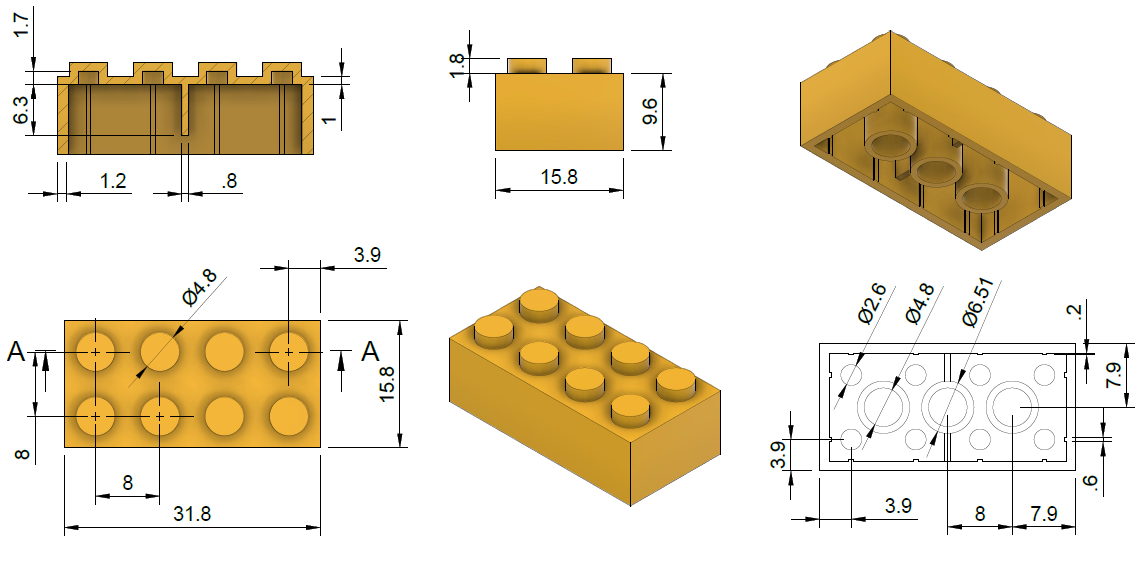
\includegraphics[width=0.8\columnwidth]{fig/LEGO 2x4 Brick horizontal.png}
    \caption{Maße des Standard 2$\times$4 LEGO Steins~\cite{LEGOBric2:online}}
    \label{fig:basics:Lego 2x4 Brick}
\end{figure}

\section{BRep}
\label{basics:brep}
Mal schauen

\section{Ontologie}
Der Begriff Ontologie stammt ursprünglich aus der Philosophie.
Wörtlich übersetzt bedeutet er \glqq{}Lehre des Seins\grqq{}.
Ein Definitionsvorschlag lautet wie folgt (aus dem Englischen):
\glqq{}Die Ontologie als Teilgebiet der Philosophie ist die Wissenschaft von dem, was existiert, den Arten und Strukturen von Objekten, Eigenschaften, Ereignissen, Prozessen und Relationen in allen Bereichen der Wirklichkeit\grqq{}~\cite{Ontology}.
Eine Anmerkung, die oftmals im Anschluss eines Definitionsvorschlags zu finden ist, besagt, dass dabei nicht nur das, \textit{was ist}, sondern ebenfalls das, \textit{was sein könnte} betrachtet werden müsse~\cite{Ontology}\cite{OntologieDefinitionLMU:online}.
Dieser Gedanke spiegelt sich ebenfalls in dem Ontologiebegriff aus der Informatik wider und ist unter dem Begriff \textit{Open World Assumption} bekannt.
Dies wird nach der Definition von Ontologien im Kontext der Informatik noch einmal ausführlicher aufgegriffen.

Im Fachbereich der Informatik wurde der Begriff Ontologie adaptiert und zunächst als \glqq{}explicit specification of a conceptualization\grqq{} definiert~\cite{Gruber1993}.
Wörtlich übersetzt lautet diese Definition etwa \glqq{}explizite Spezifizierung einer Konzeptualisierung\grqq{}.
Im Laufe der Jahre wandelte sich diese Definition, sodass sich daraus zum Beispiel folgendes ergab: \glqq{}An ontology is a formal, explicit specification of a shared conceptualization\grqq{}~\cite{Studer1998}.
Hier wird eine Ontologie also als \glqq{}formale, explizite Spezifizierung einer geteilten Konzeptualisierung\grqq{} bezeichnet.
Den wichtigsten Zusatz hierbei stellt das Wort \glqq{}geteilt\grqq{} dar, da Ontologien unter anderem dem Zweck dienen, Informationen und Vokabulare mehrerer Wissensrepräsentation zu vereinen.
Der Begriff Konzeptualisierung wird oft als \glqq{}vereinfachte, abstrakte Sicht auf einen für einen bestimmten Nutzen relevanten Teil der Welt\grqq{} beschrieben~\cite{Guarino2009}.

Eine solche \glqq{}Spezifizierung einer Konzeptualisierung\grqq{} einer gewissen Domäne kann heutzutage mithilfe der sogenannten \textit{Web Ontology Language} (OWL), welche auf dem \textit{Resource Description Framework} (RDF) aufbaut, realisiert werden~\cite{OWL_W3C}\cite{RDF_W3C}.
OWL erlaubt es Klassen zu definieren und daran Eigenschaften anzuheften.
Außerdem können sogennante Individuen beziehungsweise Instanzen erstellt werden.
Diese realisieren eine oder mehrere Klassen.
Mithilfe dieser Klassen, Eigenschaften und Individuen können sogennante \textit{Reasoner} logische Schlussfolgerungen über implizit angegebenes Wissen ziehen.
Eine Ontologie kann damit einerseits etwa mit neuen Klassenzuordnungen oder implizit angegeben Vererbungen erweitert, andererseits auf Validität überprüft werden.
Werden Verletzungen von aufgestellten Axiomem oder widersprüchliche Einschränkungen von Klassen oder Eigenschaften entdeckt, so kann ein Reasoner diese nicht nur melden, sondern auch mithilfe logischer Beweisführung herleiten.
Damit stellen Reasoner ein wertvolles Werkzeug für die Entwicklung und Erweiterung von Ontologien dar.
Drei weit verbreitete Reasoner sind: 
\begin{itemize}
  \item ELK Reasoner der Universitäten Ulm und Oxford~\cite{Kazakov2014}.
  \item HermiT Reasoner von der \textit{Information Systems Group} der Universität Oxford~\cite{Glimm2014}\cite{HermitReasoner:online}.
  \item Open Source Pellet Reasoner der Clark \& Parsia LLC~\cite{Sirin2007}. 
\end{itemize}
Aufgrund der oben genannten Idee der \textit{Open World Assumption} unterscheidet sich die Art der Reasoner logische Schlussfolgerungen zu ziehen von der, mit welcher logische Aussagen von zum Beispiel Programmiersprachen bewertet werden.
Im Grunde versteht man unter der \textit{Open World Assumption}, das nicht Falsifizieren eines logischen Ausdrucks, falls Wissen exisitieren könnte, das den Ausdruck doch verifizieren würde.
Ein Reasoner beziehungsweise eine Programmiersprache im Kontext der \textit{Closed World Assumption} würde in so einer Situation davon ausgehen alle exisitierenden Informationen darüber bereits vorliegen zu haben und eventuell zu einem anderen Schluss gelangen.
Definiert man zum Beispiel eine Klasse A als alle Individuen, die nur eine Eigenschaft E besitzen, die sie mit Individuen einer bestimmten anderen Klasse B verbindet, so kann ein Reasoner innerhalb dieser Ontologie ein Individuum, das zwar diese Anforderung erfüllt, nicht der Klasse A zuordnen, da es sein kann, dass zu einem späteren Zeitpunkt (oder an anderer Stelle) Informationen existieren, die diese Zuordnung fehlerhaft machen würden.
In einer Umgebung, in der die \textit{Closed World Assumption} gilt, wäre diese Zuordnung hingegen völlig korrekt.
Deren Annahme einer \textit{offenen Welt} ermöglicht es ebenfalls die Idee des sogenannten \glqq{}Semantic Web\grqq{} mithilfe von Ontologien zu realisieren~\cite{SemanticWebLee}.
Denn die Natur des Internets entspricht eher einer sich ständig ändernden und \glqq{}offenen\grqq{} Welt, als einer Geschlossenen.
Als Semantic Web wird das Annotieren von sämtlichen Webinhalten mit semantischen Informationen bezeichnet.
Damit wird das Ziel verfolgt, ein maschinenlesbares Internet zu schaffen. 
%TODO: da nochmal genauer drauf eingehen und semantic web kurz erwähnen -> wissen könnte ja noch iwo im internet sein, außer explizit anders angegeben.

\subsection{Protégé}
Protégé ist ein graphischer Editor zur Erstellung und Instandhaltung von Ontologien~\cite{Protege}.
Entwickelt wird das Programm an der Universität Stanford und ist als Open Source Anwendung kostenfrei nutzbar.
Die erste Version wurde bereits 1999 veröffentlicht.
Durch seine Plugin-Struktur können neben zahlreichen Erweiterungen beispielsweise auch neue Reasoner an das Programm angeschlossen werden.
Standardmäßig sind der ELK und der HermiT Reasoner integriert, aber es exisitieren Plugins um auch Pellet in Protégé zu nutzen.
Das Arbeiten mit einem graphischen Editor erleichtert den Einstieg in das Thema und ermöglicht später einen besseren Überblick über oftmals umfangreiche Ontologien, als es in einem herkömmlichen Texteditor möglich wäre.
Darum wurde das Programm zur Erstellung einer Ontologie für diese Arbeit herangezogen.

\subsection{Owlready2}
Owlready2 ist eine Python 3 Bibliothek, die es ermöglicht \glqq{}ontologie-orientiert\grqq{} zu programmieren~\cite{Owlready}.
Bisher mussten Ontologien mithilfe von Abfragesprachen (etwa SPARQL) oder APIs bearbeitet und ausgewertet werden~\cite{SPARQLF_W3C}.
Owlready2 bietet hingegen einen einfacheren Umgang mit Ontologien, ebnet damit den Einstieg in das Thema und ermöglicht gleichzeitig die Integration von Ontologien in jedes mit Python umsetzbare Projekt.
Im Zusammenspiel mit Protégé bietet diese Bibliothek eine für Programmierer intiuitive Möglichkeit, die oben genannten Werkzeuge für IFC und BIM durch Nutzung von Python 3 direkt mit der Technologie der Ontologien zu koppeln.

\section{Related Work}
\subsection{3D Druck und Additive Fertigung von Gebäuden}
\subsection{Legeroboter}
\subsection{Materialien}
\subsection{Bausteine}
\subsection{Mauer detailing und das (3D) Bin Packing Problem}
TODO hinführen über Bin Packing hin zu "spezialfall" Wall detailing mit arbiträren Bausteinen und Eigenschaften (wie versetzen der ziegel)

TODO über bin packing schreiben, erklären paper suchen, lösungsansätze zu np hartem problem 

Xu Chengran et al. haben in ihrem Paper "Optimal brick layout of masonry walls based on intelligent evolutionary algorithm and building information modeling" verschiedene Optimierungsansätze aus dem Bereich des 2D Packaging Problems getestet \cite{Xu2021}.
%TODO was ist das für ein Problem? Zitat aus nem Paper finden!
Konkret wurden drei Algorithmen verwendet: Differential Evolution, Particle Swarm Optimization und Neighbourhood Field Optimization.
%TODO ergebnisse vergleichen und eines davon hervorheben, welches ich evtl selbst einbau
Außerdem wird ein drei-phasiges Vorgehen vorgeschlagen: Data collection, Brick layout und Data Output.
%TODO das vmtl einfach auch so aufziehen. Mauern aus modell extrahieren mit geometrischen infos, optimieren und iwie rausballern
Dieses Vorgehen eignet sich auch für das Finden von Bausteinkonfigurationen in dieser Arbeit, da zuerst alle relevanten geometrischen Daten (in diesem Fall Wände, Fenster, Türen usw.) aus dem 3D Modell gesammelt werden müssen, bevor das Detailing stattfinden kann.
Nach dem Optimieren der Bausteinkonfiguration muss das Ergebnis ebenfalls in ein Format gebracht werden, das für die folgenden Schritte verwendet und eventuell auch dem Nutzer angezeigt werden kann.


Soft items: https://arxiv.org/abs/2206.15116

Irregular Shaped items: https://link.springer.com/content/pdf/10.1631/FITEE.1400421.pdf

"Parametric Blockwall-Assembly Algorithms for the Automated Generation of Virtual Wall Mockups Using BIM"

\section{Vorgehensweise}


\subsection{Einarbeiten in IFC}
Da sich IFC in der Industrie als Standard durchgesetzt hat, ist dessen Verwendung für diese Arbeit sinnvoll.
Es existieren Beispielprojekte, die zum Testen herangezogen werden können \cite{Examples1:online}.
Durch die Unterstützung von Blender können nach kurzer Einarbeitung in die Projektstruktur von IFC Modellen ebenfalls schnell eigene Projekte umgesetzt werden, die den Anforderungen besser entsprechen.

\subsection{Filtern relevanter Strukturen aus einem IFC Projekt}
Wie bereits erwähnt führt IFC Klassen wie Wände, Türen und Fenster ein. 
Dadurch sollte es möglich sein, das Modell nach Objekten zu durchsuchen, welche mit für diese Arbeit relevante Klassen markiert wurden.
Fenster und Türen stellen eine besondere Herausforderung dar, da ein Roboter, welcher auf einer Wand entlangfahren kann, vermutlich nicht in der Lage ist, diese Lücken in der Wand zu überspringen.
Somit muss das während dem Finden eines Bauplans beachtet werden.

\subsection{Diskretisieren von Strukturen mit vorgegebenen Bauteilklassen}
Es muss eine Lösung gefunden werden, beliebige Wände mit einem vorgegebenen, vermutlich stark limitierten Set an Bauteilklassen abzubilden, ohne das Modell zu verändern.
Da dies nicht immer möglich ist, wird für diese Arbeit in diesem Schritt davon ausgegangen, dass passende Modelle als Input geliefert werden, da das Einschränken des Nutzers im Modellierungsschritt stark von der Realität des Architekturprozesses abweichen würde.
Eine Möglichkeit wäre das "Teildiskretisieren" der Strukturen und ein Ausgabeset an Volumenteilen, für welche keine passende Bauteilklasse gefunden werden konnte (etwa ein Bruchteil eines Ziegels).

\subsection{Einarbeiten in und Evaluierung von Ludiwgs Dissertation}
Da Ludwigs Programmcode sehr wahrscheinlich in Teilen angepasst werden muss, ist eine Evaluierung des aktuellen Stands von Nöten und in welcher Weise dem Nutzer die darin enthaltenen Prozesse zur Verfügung gestellt werden.
Dabei könnte es sich entweder um einen in Blender integrierten Konverter handeln oder um eine Erweiterung des BIM-Servers.
Außerdem gilt es herauszufinden, ob das Anpassen seines Algorithmus an für Roboterschwärme optimierte Baupläne den Rahmen dieser Arbeit sprengen würde und wie sich dessen Output dafür ändern müsste.
Eventuell ist es ausreichend, den Roboterschwarm nicht bei der Suche nach einem geeigneten Bauplan zu berücksichtigen und diesen sogar dahingehend zu optimieren, sondern im Anschluss den Bauplan nach Möglichkeiten zur synchronen Bearbeitung mehrerer Agenten zu untersuchen.

\subsection{Überführung in Ludwigs Format}
Nach der Diskretisierung des Modells in eine Menge an Bauteilen, können diese in das von Ludwigs Dissertation vorgesehene Schema konvertiert werden.
Dazu müssen vor allem die Beziehungen einzelner Bauteile zueinander erkannt und die Constraints der Bauteilklassen und Robotertypen beachtet werden.
Im Anschluss können diese Daten nun verwendet werden, um mithilfe von Ludiwgs Dissertation einen Bauteilplan zu suchen.

\subsection{Format des Ergebnisses festlegen}
Hier müsssen sich Luca und ich über den Verlauf unserer Masterarbeiten immer wieder absprechen und Anforderungen vergleichen.


\medskip

\printbibliography
\end{document}

%%%%%%%%%%%%%%%%%%%%%%%%%%%%%%%%%%%%%%%%

% Copyright Remarks:
%--------------------

% Copyright holder: Vebjørn S. Førde, copyright: CC BY 4.0
% Note: The author of this template is also the copyright holder.

% Below is an explanation of the CC BY 4.0. Additional statements/ 
% clarifications made by the author/copyright holder are marked with *.

% YOU ARE FREE TO:
% Share — copy and redistribute the material in any medium or format
% Adapt — remix, transform, and build upon the material
% for any purpose, even commercially.

% UNDER THE FOLLOWING TERMS:
% Attribution* — You must give appropriate credit, provide a link to the license,
% and indicate if changes were made. You may do so in any reasonable manner, but 
% not in any way that suggests the licensor endorses you or your use.

% *Note: 
% Attribution NOT NEEDED for: 
%       - PDF distibution (like sharing your PDF document)
%       - Use of (dummy)text and images provided in the template (obviously)
%       - Distributing parts of the template, and not the template as a whole
% I am not really concerned with being given credit. As long as you do not 
% claim to have made the template yourself in distributing it further, I have
% no complaints.

% No additional restrictions — You may not apply legal terms or technological 
% measures that legally restrict others from doing anything the license permits.

% NOTICES:
% No warranties are given.

% Disclaimer* (added by copyright holder):
% THE SOFTWARE IS PROVIDED "AS IS", WITHOUT WARRANTY OF ANY KIND, EXPRESS OR
% IMPLIED, INCLUDING BUT NOT LIMITED TO THE WARRANTIES OF MERCHANTABILITY,
% FITNESS FOR A PARTICULAR PURPOSE AND NONINFRINGEMENT. IN NO EVENT SHALL THE
% AUTHORS OR COPYRIGHT HOLDERS BE LIABLE FOR ANY CLAIM, DAMAGES OR OTHER
% LIABILITY, WHETHER IN AN ACTION OF CONTRACT, TORT OR OTHERWISE, ARISING FROM,
% OUT OF OR IN CONNECTION WITH THE SOFTWARE OR THE USE OR OTHER DEALINGS IN THE
% SOFTWARE.

% Read more about CC BY 4.0:
% https://creativecommons.org/licenses/by/4.0/